\documentclass[12pt,a4paper]{report}
\usepackage[utf8]{inputenc}
\usepackage[T1]{fontenc}
\usepackage{geometry}
\geometry{a4paper, margin=1in}
\usepackage[table]{xcolor}
\usepackage{graphicx}
\usepackage{fancyhdr}
\usepackage{hyperref}
\usepackage{tabularx}
\usepackage{array}
\usepackage{float}
\usepackage{amsmath}
\usepackage{tikz}
\usepackage{titlesec}
\usepackage{setspace}
\usepackage{lipsum} % For testing and filling space if needed

\pagestyle{fancy}
\fancyhf{}
\setlength{\headheight}{14.5pt}
\addtolength{\topmargin}{-2.5pt}
\fancyhead[L]{TETE3109 - Comprehensive Review}
\fancyhead[R]{Maintenance \& Data Systems}
\fancyfoot[C]{\thepage}

\begin{document}

\begin{titlepage}
    \singlespacing
    \centering
    \vspace*{0.3cm}
    
    % University Crest
    
\includegraphics[height=2.7cm]{kyu_crest.png} \\[0.6cm]
    
    % University Name & Department
    {\LARGE \textbf{KYAMBOGO UNIVERSITY}} \\[0.3cm]
    {\small \textsc{Department of Electrical and}} \\[0.15cm]
    {\small \textsc{Electronics Engineering Faculty of}} \\[0.15cm]
    {\small \textsc{Engineering}} \\[1.5cm]
    
    % Course Code & Title
    {\LARGE \textbf{TETE3109}} \\[0.35cm]
    {\Large \textbf{Maintenance and Data Systems}} \\[0.25cm]
    {\large Chapter 8 -- Comprehensive Review} \\[1.1cm]
    
    % Assignment Details
    {\large \textbf{Group 4 Assignment}} \\[0.4cm]
    {\large Lecturer: Dr.~Ephrance Eunice Namugenyi} \\[1.2cm]
    
    % Horizontal rule above table
    {\color[HTML]{999999}\rule{9.2cm}{0.5pt}} \\[0.25cm]
    
    % Table of Members
    \renewcommand{\arraystretch}{1.55}
    \setlength{\tabcolsep}{10pt}
    \begin{tabular}{>{\raggedleft\arraybackslash\itshape}p{5.0cm} !{\color[HTML]{BEBEBE}\vrule width 0.6pt} >{\raggedright\arraybackslash}p{8.4cm}}
        \multicolumn{1}{p{5.0cm}}{\raggedleft\textit{Student Name}} & 
        \multicolumn{1}{p{8.4cm}}{\raggedright\textit{Registration / Student No.}} \\
        \arrayrulecolor[HTML]{BEBEBE}\hline
        Wabwire Harrison & \cellcolor[HTML]{F1F1F1} 24/U/ETD/1857/PD \\
        Aliu Gabriel & 24/U/ETE/02970/PE \\
        Kidega Wilkie Cephas & \cellcolor[HTML]{F1F1F1} 25/U/ETE/05460/PE \\
        Oyana Andrew Benard & 25/U/ETD/00812/GV \\
        Ainembabazi Godwin & \cellcolor[HTML]{F1F1F1} 26/U/ETE/21277/PE \\
    \end{tabular}
    
    \vspace*{\fill}
    
    % Date at bottom left
    \begin{flushleft}
        {\large September 28, 2026}
    \end{flushleft}
\end{titlepage}

\begingroup
\singlespacing
\makeatletter
\renewcommand*\l@chapter[2]{%
  \ifnum \c@tocdepth >\m@ne
    \addpenalty{-\@highpenalty}%
    \vskip 0.4em \@plus\p@
    \setlength\@tempdima{1.5em}%
    \begingroup
      \parindent \z@ \rightskip \@pnumwidth
      \parfillskip -\@pnumwidth
      \leavevmode \bfseries
      \advance\leftskip\@tempdima
      \hskip -\leftskip
      #1\nobreak\hfil \nobreak\hb@xt@\@pnumwidth{\hss #2}\par
      \penalty\@highpenalty
    \endgroup
  \fi}
\makeatother
\tableofcontents
\endgroup
\clearpage

% Merged List of Figures and List of Tables on a single page
\begingroup
\singlespacing
\let\clearpage\relax
\let\cleardoublepage\relax
\vspace*{-0.5cm}
\listoffigures
\vspace{1.5cm}
\listoftables
\endgroup
\clearpage

% List of Abbreviations and Short Terms with Full Definitions
\chapter*{List of Abbreviations and Short Terms}
\addcontentsline{toc}{chapter}{List of Abbreviations and Short Terms}
\markboth{List of Abbreviations and Short Terms}{List of Abbreviations and Short Terms}

This section provides formal expansions and comprehensive technical definitions for all abbreviations, acronyms, and shorthand terms used throughout this document.

\vspace{0.3cm}

\noindent\textbf{AC (Alternating Current):} An electric current whose magnitude and direction vary cyclically over time. In analog local subscriber loops, a high-voltage AC signal (typically $75\text{--}90\text{V AC}$ at $20\text{--}25\text{ Hz}$) is sent by the central office exchange to actuate the electromechanical bell or ringer in the subscriber's telephone handset.

\vspace{0.2cm}
\noindent\textbf{AI (Artificial Intelligence):} The simulation of human intelligence by computer systems. In telecommunication data systems, AI algorithms are applied to analyze network telemetry, predict traffic congestion, optimize dynamic routing, and detect cybersecurity anomalies.

\vspace{0.2cm}
\noindent\textbf{AIOps (Artificial Intelligence for IT Operations):} The integration of artificial intelligence, machine learning, and big data analytics into network operations. AIOps platforms automate fault localization, performance analysis, root-cause diagnostics, and self-healing remediations across modern telecom architectures.

\vspace{0.2cm}
\noindent\textbf{ASCII (American Standard Code for Information Interchange):} A standard 7-bit (or 8-bit extended) character encoding scheme. In asynchronous serial dial-up communications, each character is framed by 1 start bit, 8 data bits, and 1 stop bit (yielding 10 bits total per character frame).

\vspace{0.2cm}
\noindent\textbf{ASR (Answer-Seizure Ratio):} A primary telecommunications quality-of-service (QoS) metric that measures the percentage of call seizure attempts that result in an answered call:
\[ \text{ASR} = \left(\frac{\text{Total Answered Calls}}{\text{Total Call Seizures}}\right) \times 100\% \]
A degraded ASR indicates network congestion, transmission line failures, or unallocated dialed numbers.

\vspace{0.2cm}
\noindent\textbf{AXE (Automatic Crossbar Electronic):} A family of modular digital electronic telephone switching systems developed by Ericsson. AXE switches serve as public Class 4 (tandem) and Class 5 (local) exchanges capable of routing high-volume digital voice and signaling traffic.

\vspace{0.2cm}
\noindent\textbf{BER (Bit Error Rate):} The ratio of received data bits that have been altered or corrupted due to noise, interference, distortion, or attenuation relative to the total number of transmitted bits over a digital communication link. It serves as a key performance indicator (KPI) for predictive physical-layer maintenance.

\vspace{0.2cm}
\noindent\textbf{BHCA (Busy Hour Call Attempts):} A telecommunication capacity engineering metric representing the peak number of call setup attempts an exchange processor can handle during its most heavily loaded 60-minute interval (the busy hour).

\vspace{0.2cm}
\noindent\textbf{bps / kbps / Mbps (Bits, Kilobits, Megabits per second):} Units of digital data transmission speed indicating the number of binary bits transferred across a communication channel per second ($1\text{ kbps} = 10^3\text{ bps}$, $1\text{ Mbps} = 10^6\text{ bps}$).

\vspace{0.2cm}
\noindent\textbf{BSS (Business Support Systems):} The collection of enterprise software and database systems that handle customer-facing commercial operations for a telecom operator, including customer relationship management (CRM), billing and rating, product cataloging, order fulfillment, revenue assurance, and fraud management.

\vspace{0.2cm}
\noindent\textbf{CDR (Call Detail Record):} A structured data record generated by a telephone exchange, softswitch, or IP gateway at the termination of a call. It logs call attributes including caller and called numbers, start time, duration, call disposition, and network routes for accounting and billing purposes.

\vspace{0.2cm}
\noindent\textbf{Cisco Troubleshooting Model:} A structured six-phase diagnostic methodology used to systematically isolate and resolve technical network faults: (1) Identify the problem, (2) Theorize probable cause, (3) Test the theory, (4) Implement the plan of action, (5) Verify system functionality, and (6) Document findings.

\vspace{0.2cm}
\noindent\textbf{CRM (Customer Relationship Management):} Enterprise platforms used by telecommunications carriers to manage subscriber accounts, track service requests, log customer support tickets, and administer client lifecycle services.

\vspace{0.2cm}
\noindent\textbf{DC (Direct Current):} Unidirectional flow of electrical charge. In telephony, central office battery banks supply a continuous $-48\text{V DC}$ voltage across the subscriber loop to power terminal equipment and sense off-hook loop current.

\vspace{0.2cm}
\noindent\textbf{DP (Distribution Point):} The physical termination box (e.g., DP3) on an external telephone pole or building wall that interconnects the multi-pair distribution cable from the exchange with individual subscriber drop wires.

\vspace{0.2cm}
\noindent\textbf{DTMF (Dual-Tone Multi-Frequency):} An in-band signaling technique used for touch-tone telephone dialing. Pressing a telephone keypad key simultaneously generates two sinusoidal tones (one low group frequency and one high group frequency) representing the selected digit.

\vspace{0.2cm}
\noindent\textbf{E1 Standard:} The European digital carrier transmission hierarchy standard standardized by ITU-T (G.703/G.704) operating at $2.048\text{ Mbps}$. An E1 frame multiplexes 32 time slots of $64\text{ kbps}$ each: 30 time slots carry user voice/data, time slot 0 is reserved for framing/synchronization, and time slot 16 carries out-of-band signaling.

\vspace{0.2cm}
\noindent\textbf{E.164:} The international public telecommunication numbering plan established by the ITU-T. It specifies the global hierarchical telephone numbering format (comprising country code, national destination code, and subscriber number) up to a maximum length of 15 digits.

\vspace{0.2cm}
\noindent\textbf{EWSD (Elektronisches W\char"00E4hlsystem Digital):} A globally deployed digital electronic telephone switching system designed by Siemens, utilized worldwide as public Class 4 transit and Class 5 local telephone exchanges.

\vspace{0.2cm}
\noindent\textbf{FCAPS:} The ISO telecommunications network management model that categorizes network management into five core disciplines:
\begin{itemize}
    \item \textbf{Fault Management (F):} Detection, logging, isolation, and resolution of equipment and link failures.
    \item \textbf{Configuration Management (C):} Hardware/software inventory tracking, service provisioning, and configuration version control.
    \item \textbf{Accounting Management (A):} Measurement of network usage and collection of CDRs for billing and resource auditing.
    \item \textbf{Performance Management (P):} Real-time monitoring of metrics such as latency, throughput, packet loss, CPU load, and traffic intensity (Erlangs).
    \item \textbf{Security Management (S):} Authentication, authorization, access control, encrypted management channels, and fraud detection.
\end{itemize}

\vspace{0.2cm}
\noindent\textbf{Friis Formula:} An analytical formula used in RF and telecommunications engineering to calculate the total cascaded noise figure of multi-stage amplifier systems, demonstrating that the noise figure of the first stage (e.g., LNA) dominates overall system noise.

\vspace{0.2cm}
\noindent\textbf{G.711:} The ITU-T audio companding standard that digitizes voice over $64\text{ kbps}$ channels by sampling at $8,000\text{ samples/s}$ with 8-bit logarithmic quantization using either A-law (Europe/Africa) or $\mu$-law (North America/Japan).

\vspace{0.2cm}
\noindent\textbf{IAM (Initial Address Message):} The primary call setup message in the ISDN User Part (ISUP) of Signaling System No. 7 (SS7). It is transmitted across signaling links to seize a voice trunk circuit and transfer the dialed destination digits to the next exchange.

\vspace{0.2cm}
\noindent\textbf{IMS (IP Multimedia Subsystem):} An architectural framework standardized by 3GPP for delivering multimedia and voice communications over Internet Protocol (IP) networks, enabling seamless multimedia services across fixed, mobile (4G/5G), and wireless access networks.

\vspace{0.2cm}
\noindent\textbf{INVITE:} The primary request method in the Session Initiation Protocol (SIP, RFC 3261) sent by an originating user agent or gateway to initiate a voice or video media session with a recipient.

\vspace{0.2cm}
\noindent\textbf{IP (Internet Protocol):} The core network-layer protocol of the Internet suite that routes discrete data packets across network boundaries based on logical IP addresses.

\vspace{0.2cm}
\noindent\textbf{LNA (Low-Noise Amplifier):} A specialized high-sensitivity amplifier positioned at the front-end antenna receiver of RF, microwave, and satellite links designed to amplify faint incoming signals while contributing minimal intrinsic noise.

\vspace{0.2cm}
\noindent\textbf{MTBF (Mean Time Between Failures):} A statistical reliability metric measuring the average operational time elapsed between successive hardware or system failures during normal operational conditions.

\vspace{0.2cm}
\noindent\textbf{MTTR (Mean Time To Repair):} The average duration required to troubleshoot, repair or replace, and restore a failed network component back into active operational service.

\vspace{0.2cm}
\noindent\textbf{NMS (Network Management System):} Centralized software and hardware platforms used in Network Operations Centers (NOCs) to monitor, configure, analyze, and manage active telecommunications infrastructure.

\vspace{0.2cm}
\noindent\textbf{OSS (Operations Support Systems):} Network-facing software applications that support operational telecom activities, including network inventory, service provisioning, fault resolution, network monitoring, and field maintenance dispatch.

\vspace{0.2cm}
\noindent\textbf{OTDR (Optical Time-Domain Reflectometer):} An optoelectronic instrument used to diagnose and verify optical fibers by transmitting laser pulses down a fiber core and measuring Rayleigh backscatter and Fresnel reflections to locate splices, connectors, and physical breaks.

\vspace{0.2cm}
\noindent\textbf{PBX (Private Branch Exchange):} An internal telephone switching exchange owned and operated by an enterprise or campus that switches calls internally between office extensions and routes external calls across public telephone trunks.

\vspace{0.2cm}
\noindent\textbf{PCM (Pulse Code Modulation):} The foundational digital modulation technique used to convert analog signals into digital binary code through three sequential stages: Nyquist sampling, non-linear quantization, and binary encoding.

\vspace{0.2cm}
\noindent\textbf{PSTN (Public Switched Telephone Network):} The worldwide interconnected circuit-switched telecommunications network operated by national and commercial service providers, providing public voice connectivity via copper, fiber, and microwave transmission systems.

\vspace{0.2cm}
\noindent\textbf{SIP (Session Initiation Protocol):} An application-layer text-based signaling protocol (RFC 3261) used for establishing, modifying, and terminating interactive real-time communication sessions such as Voice over IP (VoIP) and video calls.

\vspace{0.2cm}
\noindent\textbf{SNMP (Simple Network Management Protocol):} An established application-layer protocol used to collect telemetry, monitor device operational metrics, and configure network hardware (routers, switches, servers) via managed MIB variables.

\vspace{0.2cm}
\noindent\textbf{SS7 (Signalling System No. 7):} An international suite of telephony signaling protocols developed by ITU-T that operates out-of-band on a dedicated data network to perform call setup, routing, billing, and teardown across circuit-switched telephone exchanges.

\vspace{0.2cm}
\noindent\textbf{Syslog:} A standard event logging protocol allowing network devices and telephony servers to forward system error logs, status messages, and operational alerts over an IP network to a central log repository.

\vspace{0.2cm}
\noindent\textbf{TETE:} The academic departmental course prefix for Telecommunication Engineering at Kyambogo University (e.g., TETE3109: Maintenance and Data Systems).

\vspace{0.2cm}
\noindent\textbf{UCC (Uganda Communications Commission):} The national statutory regulatory authority established under the Uganda Communications Act to regulate, license, and develop telecommunications, radio frequency spectrum, and broadcasting in Uganda.

\vspace{0.2cm}
\noindent\textbf{VoIP (Voice over Internet Protocol):} A suite of technologies enabling the digitization, packetization, and transmission of voice telephone calls across packet-switched IP networks instead of legacy circuit-switched PSTN lines.

\vspace{0.2cm}
\noindent\textbf{VoLTE (Voice over Long-Term Evolution):} A carrier-grade, packet-switched high-definition voice service standard that operates natively over 4G LTE cellular data networks using an IMS core with dedicated Quality of Service (QoS).

\vspace{0.2cm}
\noindent\textbf{VoNR (Voice over New Radio):} The native packet-switched voice communication architecture for 5G Standalone (SA) mobile networks, processing voice calls directly on the 5G core network without requiring 4G LTE fallback.

\clearpage
\onehalfspacing

\chapter{Introduction to Data Systems}

\section{What is a Data System?}
A data system is an organized infrastructure that collects, stores, processes, and presents data to make informed decisions. It can be viewed as an arrangement of a source, medium, and destination that captures information, converts it into signals, moves those signals across a channel, and reconstructs the original information at the far end reliably.

\subsection{Key Components}
\begin{itemize}
    \item \textbf{Source:} Generates data (voice, text, image, sensor reading).
    \item \textbf{Transmitter:} Encodes and modulates the data onto a signal.
    \item \textbf{Channel:} The medium of transmission (wire, air, fibre).
    \item \textbf{Receiver/Sink:} Demodulates and reconstructs the original data.
\end{itemize}

\subsection{The 4 Functions of a Data System}
\begin{enumerate}
    \item \textbf{COLLECT:} Gathers raw data using SNMP agents, CDR generators, Syslogs, and OTDR sensors.
    \item \textbf{STORE:} Retains data in Databases (MySQL, Oracle) and Data Lakes (Hadoop).
    \item \textbf{PROCESS:} Analyzes data through mediation, correlation, normalization, and AI prediction.
    \item \textbf{PRESENT:} Displays information via NMS dashboards, billing invoices, and Grafana reports.
\end{enumerate}

Analogy: If voice transmission represents the goods sold in a shop, the Data System is the cashier, stock book, CCTV, and manager working together to ensure smooth operation. In telephony, every call creates data; without a data system, there is no billing, fault detection, or planning.

\chapter{The Telephone System}

\section{Telephone System Overview}
The Telephone System is an integrated, carrier-grade network enabling bidirectional real-time voice communication between dispersed subscribers via synchronized switching, transmission, and signaling subsystems. Historically, the telephone network represents mankind's first continental-scale automated data system, pioneering principles of circuit switching, network hierarchy, centralized management, and computerized billing.

\subsection{Five Pillars of Telephony}
A complete telecommunications system relies on five foundational subsystems:
\begin{itemize}
    \item \textbf{Terminals (User Equipment):} Subscriber endpoints that convert acoustic energy into electrical or digital signals. These span legacy analog dual-tone multi-frequency (DTMF) telephone sets, Session Initiation Protocol (SIP) desktop IP phones, and modern multi-mode smartphones supporting 2G/3G/4G/5G New Radio (NR) interfaces.
    \item \textbf{Transmission Media:} Physical and wireless propagation channels transporting modulated voice and data signals. In modern carrier architectures, transmission encompasses subterranean and aerial single-mode optical fiber (carrying DWDM aggregates), line-of-sight point-to-point microwave radio links (e.g., $7\text{--}38\text{ GHz}$ backhauls), and cellular radio access frequencies.
    \item \textbf{Switching and Routing Engines:} Centralized intelligent nodes responsible for interpreting dialed digits, identifying destination paths, establishing physical or virtual connections, and releasing resources upon call termination. This evolved from electro-mechanical crossbar switches to electronic digital Class 4/5 exchanges (e.g., Siemens EWSD, Ericsson AXE) and contemporary cloud-native Softswitches, IP Multimedia Subsystem (IMS) cores, and Voice over LTE/NR gateways.
    \item \textbf{Signaling Subsystems:} Dedicated control networks operating out-of-band to orchestrate call setup, routing, status verification, feature invocation, and call teardown. Core protocols include Signaling System No.~7 (SS7 / C7) in circuit-switched networks and Session Initiation Protocol (SIP / RFC 3261) in packet-switched IP networks.
    \item \textbf{Telecommunications Data Systems (Management \& OSS/BSS):} The administrative nervous system comprising Network Operations Centers (NOC), Network Management Systems (NMS), Operations Support Systems (OSS), and Business Support Systems (BSS) that handle real-time fault monitoring, performance metrics, convergent prepaid rating, billing mediation, and regulatory reporting.
\end{itemize}

\subsection{Evolution of Switching Technology}
The architectural evolution of telephony switching spans seven distinct historical generations:
\begin{enumerate}
    \item \textbf{Manual Patchboards:} Operator-manned cords connecting jacks on switchboards.
    \item \textbf{Strowger Step-by-Step:} Electromechanical two-motion rotary step switches.
    \item \textbf{Electromechanical Crossbar:} Coordinate matrix switches controlled by common markers.
    \item \textbf{Stored Program Control (SPC) Digital:} Computer-controlled digital switching (e.g., Siemens EWSD, Ericsson AXE).
    \item \textbf{VoIP Softswitch:} Decoupled call control and IP media gateways (SIP / H.323).
    \item \textbf{IP Multimedia Subsystem (IMS / VoLTE):} All-IP SIP multimedia core with dedicated QoS over cellular 4G LTE.
    \item \textbf{5G Cloud-Native SBA (VoNR):} Microservices and Service-Based Architecture for native 5G voice.
\end{enumerate}

\section{PSTN Architecture and Public Switching Hierarchy}
The Public Switched Telephone Network (PSTN) is the worldwide collection of interconnected circuit-switched and IP-based public telephone networks. In traditional telecommunications engineering, PSTN switching is structured in a strict hierarchical pyramid designed to optimize transmission costs and prevent call blocking:
\begin{itemize}
    \item \textbf{Class 5 (Local Exchange / End Office):} Connects subscriber local loops directly (typically serving 1,000 to 50,000 subscriber lines). It delivers dial tone, applies $-48\text{V DC}$ talk battery, injects $75\text{V AC}$ ringing current, interprets dialed DTMF digits, and marks the originating timestamp for Call Detail Records (CDRs).
    \item \textbf{Class 4 (Tandem / Junction Exchange):} High-capacity intermediate switching centers that interconnect multiple Class 5 local exchanges within a common metropolitan area. Tandems do not terminate subscriber loops; their sole role is inter-exchange traffic concentration and routing.
    \item \textbf{Class 3 and Class 2 (Primary and Secondary Toll Centers):} National transit switches that aggregate inter-city long-distance traffic across regional trunk groups.
    \item \textbf{Class 1 (Regional / International Gateway):} Massive transit exchanges connected to international undersea fiber optic cable landing stations (e.g., submarine landing stations along the East African coast) and international satellite gateways, routing overseas calls via the ITU-T E.164 international numbering framework.
\end{itemize}

\section{The Ugandan Telecommunications Landscape: MTN, Airtel, and the UCC Framework}
The structure of telecommunications in Uganda presents a unique and compelling study in network evolution. Unlike North American and Western European markets that operated massive copper-based fixed-line PSTN infrastructure for over a century, Uganda experienced a rapid technological leapfrog directly into cellular mobile telephony and fiber backbones.

\subsection{The Regulatory Framework: Uganda Communications Commission (UCC)}
Telecommunications in Uganda is governed by the \textbf{Uganda Communications Commission (UCC)}, established under the Uganda Communications Act 2013 (originally promulgated in 1997 following the unbundling of the state monopoly, Uganda Posts and Telecommunications Corporation - UPTC). The UCC administers:
\begin{itemize}
    \item \textbf{Radio Frequency Spectrum Licensing:} Allocating and monitoring frequencies across mobile access bands (700 MHz, 800 MHz, 900 MHz, 1800 MHz, 2100 MHz, 2.3 GHz, 2.6 GHz, and 3.5 GHz) and microwave backhaul links.
    \item \textbf{Interconnection Regulations and Interconnect Usage Charges (IUC):} Setting the regulatory cost-based glide path for cross-network call termination rates between licensed operators (mandated at approximately UGX 35 per minute for voice).
    \item \textbf{Quality of Service (QoS) Benchmarks:} Enforcing strict quarterly drive-test compliance across all 135 districts of Uganda for metrics including Call Setup Success Rate (CSSR $\ge 98\%$) and Call Drop Rate (CDR $\le 1\%$).
    \item \textbf{National Numbering Plan (E.164):} Allocating national destination codes (NDCs) and short codes to licensed public telecommunication operators.
    \item \textbf{Mandatory SIM Card Registration:} Enforcing the linkage of every active SIM card with verified National Identification Numbers (NIN) via direct real-time API queries to the National Identification and Registration Authority (NIRA) database.
\end{itemize}

\subsection{Major Mobile Network Operators (MNOs) in Uganda}
The Ugandan commercial telephony market is characterized by an operational duopoly anchored by two multinational telecommunications operators:
\begin{enumerate}
    \item \textbf{MTN Uganda (Mobile Country Code 641, MNC 10):}
    Launched commercial operations in October 1998, pioneering affordable prepaid telecommunications, electronic voucher recharge, and per-second billing. Today, MTN Uganda commands the largest market share (over $53\%$, representing approximately 19 million subscribers). MTN operates two primary Tier-3 Core Switching and Data Centers: the \textbf{Mutundwe Data Center} (primary core switching, IMS, and IT data center) and the \textbf{Bugolobi Data Center} (secondary geographic redundancy and metro transmission hub). MTN maintains a nationwide Dense Wavelength Division Multiplexing (DWDM) optical fiber transmission backbone linking Kampala with border crossing points at Malaba/Busia (Kenya), Katuna/Mirama Hills (Rwanda), Mutukula (Tanzania), and Elegu (South Sudan).
    
    \item \textbf{Airtel Uganda (Mobile Country Code 641, MNC 01):}
    Traces its origins to \textbf{Celtel Uganda}, which established the country's first commercial cellular network in 1995. The company transitioned through Zain Uganda before its acquisition by Bharti Airtel in 2010. Airtel strengthened its competitive positioning through two major market consolidations: the acquisition and merger with \textbf{Warid Telecom Uganda} in 2013 (which significantly expanded its subscriber base and urban footprint) and the acquisition of the operational assets and spectrum of \textbf{Africell Uganda} following its market exit in 2021. Airtel serves over $43\%$ of the Ugandan market (over 14 million subscribers), operating its primary mobile switching centers and packet cores at \textbf{Clement Hill Road} and \textbf{Bugolobi} in Kampala.
    
    \item \textbf{Other Operators and Infrastructure Providers:}
    \begin{itemize}
        \item \textit{Uganda Telecom Limited (UTL / UTCL):} The state-owned telecommunications enterprise resulting from the privatization of UPTC. UTL owns substantial legacy copper outside plant, fixed enterprise fiber, government administrative telephony lines, and a national transit switching center in central Kampala.
        \item \textit{Lycamobile Uganda (MNC 26):} A Mobile Virtual Network Operator (MVNO) / National Operator providing high-speed mobile data and competitive VoIP/voice services.
        \item \textit{American Tower Corporation (ATC Uganda):} An independent passive telecommunications infrastructure provider. Following infrastructure carve-outs by both MTN and Airtel, ATC owns, manages, and maintains over $4,000$ passive tower sites across Uganda. ATC leases tower verticality, aviation lighting, physical compound security, and hybrid backup power (diesel generators, solar photovoltaic arrays, and $48\text{V}$ battery banks) to MTN, Airtel, and public security agencies.
    \end{itemize}
\end{enumerate}

\subsection{The Leapfrogging Phenomenon in Ugandan Telephony}
In developed Western economies, national carriers invested billions of dollars across the 20th century burying hundreds of thousands of kilometers of paper-insulated and polyethylene-insulated copper multipair cables to every household and business. When mobile networks emerged, they were built as an overlay to an existing, universal fixed PSTN.

In Uganda, geographical dispersion, low initial rural income, high outside plant maintenance costs, and frequent copper vandalism prevented the nationwide rollout of copper local access loops outside major institutional centers. By the year 2000, fixed-line telephone penetration in Uganda lingered at less than $0.3\%$. The rapid deployment of cellular GSM (and subsequently 3G, 4G LTE, and 5G NR) completely bypassed the copper era:
\begin{itemize}
    \item Fixed-line teledensity remains below $0.5\%$ of the population.
    \item Mobile cellular teledensity exceeds $72\%$, with over 34 million connected SIM cards nationwide.
    \item Fixed enterprise communication is delivered almost exclusively via direct Gigabit Passive Optical Network (GPON) fiber to the business or fixed-wireless point-to-multipoint microwave links, while consumer voice is dominated by mobile VoLTE and 2G/3G circuit-switched cellular.
\end{itemize}

\chapter{Journey of a Call (A to Z)}

\section{Classical Call Flow: House A to House B}
To understand switching and data operations, consider the sequential progression of an analog landline call between two subscribers (House A and House B) connected through local exchanges and an intermediate tandem:

\begin{figure}[H]
\centering
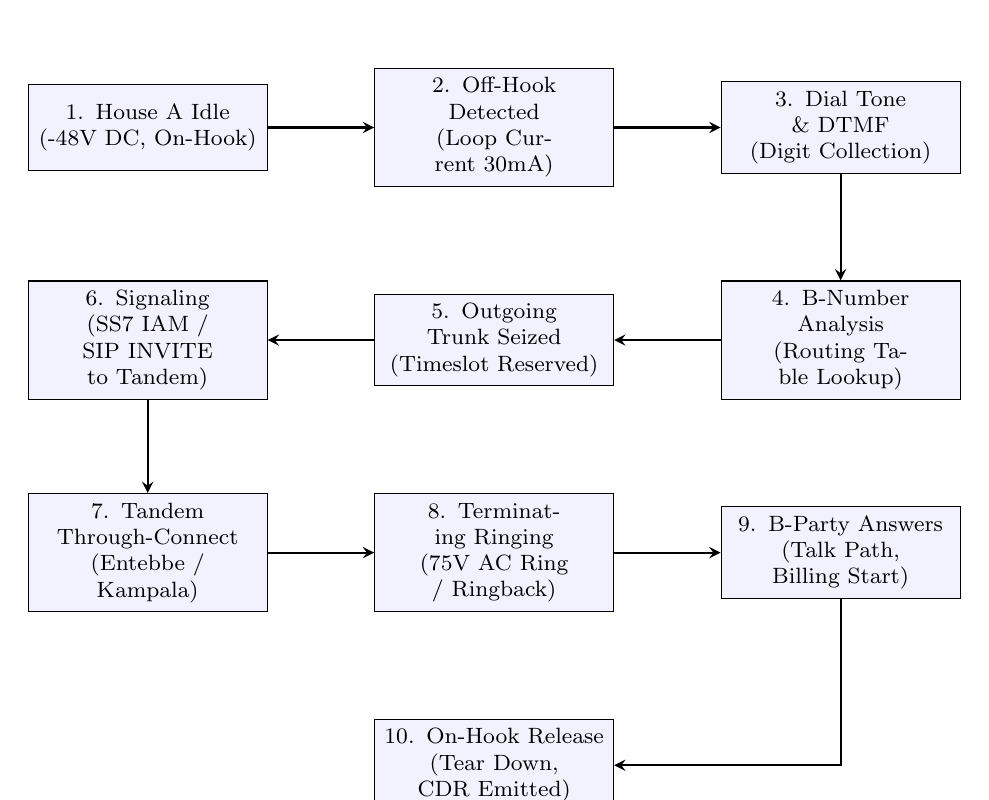
\begin{tikzpicture}[node distance=2.2cm, auto, >=stealth]
\tikzstyle{block} = [draw, rectangle, fill=blue!5, text width=2.8cm, text centered, minimum height=1.1cm, font=\footnotesize]
\tikzstyle{line} = [draw, ->, thick]

\node [block] (A) {1. House A Idle\\(-48V DC, On-Hook)};
\node [block, right of=A, xshift=2.2cm] (B) {2. Off-Hook Detected\\(Loop Current 30mA)};
\node [block, right of=B, xshift=2.2cm] (C) {3. Dial Tone \& DTMF\\(Digit Collection)};
\node [block, below of=C, yshift=-0.5cm] (D) {4. B-Number Analysis\\(Routing Table Lookup)};
\node [block, left of=D, xshift=-2.2cm] (E) {5. Outgoing Trunk Seized\\(Timeslot Reserved)};
\node [block, left of=E, xshift=-2.2cm] (F) {6. Signaling (SS7 IAM /\\SIP INVITE to Tandem)};
\node [block, below of=F, yshift=-0.5cm] (G) {7. Tandem Through-Connect\\(Entebbe / Kampala)};
\node [block, right of=G, xshift=2.2cm] (H) {8. Terminating Ringing\\(75V AC Ring / Ringback)};
\node [block, right of=H, xshift=2.2cm] (I) {9. B-Party Answers\\(Talk Path, Billing Start)};
\node [block, below of=H, yshift=-0.5cm] (J) {10. On-Hook Release\\(Tear Down, CDR Emitted)};

\path [line] (A) -- (B);
\path [line] (B) -- (C);
\path [line] (C) -- (D);
\path [line] (D) -- (E);
\path [line] (E) -- (F);
\path [line] (F) -- (G);
\path [line] (G) -- (H);
\path [line] (H) -- (I);
\path [line] (I) |- (J);
\end{tikzpicture}
\caption{Classical Circuit-Switched Call Flow Architecture}
\label{fig:classical_call_flow}
\end{figure}

\begin{enumerate}
    \item \textbf{Idle State:} Handset on-hook. Exchange line card applies a steady $-48\text{V DC}$ talk battery across Tip and Ring conductors. The circuit is open; only a minute microampere leakage current flows.
    \item \textbf{Off-Hook Detection:} Lifting the handset closes the cradle switch contacts, completing the DC loop through the hybrid coil. A continuous loop current of $20\text{--}40\text{ mA}$ flows. The exchange sense relay trips, marking the line as active.
    \item \textbf{Dial Tone \& Dialing:} The local exchange attaches a DTMF digit receiver and transmits a dual-frequency continuous dial tone ($350\text{ Hz} + 440\text{ Hz}$). The caller dials the subscriber number. Keypresses generate pairwise DTMF tones collected in the exchange register.
    \item \textbf{Routing and Digit Analysis:} The central processor performs longest-prefix matching against routing tables to determine whether the call is local to the exchange, inter-exchange, or national toll.
    \item \textbf{Trunk Seizure:} An available outgoing voice channel (time slot on an E1 carrier or IP packet bearer) is seized.
    \item \textbf{Out-of-Band Signaling:} The originating exchange formats an SS7 Initial Address Message (IAM) or SIP `INVITE` message containing the Calling Party Number (A-number) and Called Party Number (B-number), transmitting it across signaling links.
    \item \textbf{Tandem Switching:} The tandem exchange analyzes the destination address and through-connects the signaling and bearer channels to the terminating local exchange.
    \item \textbf{Terminating Ringing and Ring-Back:} The terminating exchange checks the B-party line state:
    \begin{itemize}
        \item If busy, a Busy Tone ($480\text{ Hz} + 620\text{ Hz}$, 0.5s on / 0.5s off) is returned to House A.
        \item If idle, the exchange injects a high-voltage $75\text{V AC}$ ringer current at $25\text{ Hz}$ cadenced (1s ring, 2s silence) across House B's line, while simultaneously returning an audible Ring-Back Tone ($440\text{ Hz} + 480\text{ Hz}$) to House A.
    \end{itemize}
    \item \textbf{Answer and Conversation:} House B lifts the handset. Current flow trips the ringing generator. An SS7 Answer Message (ANM) or SIP `200 OK` is returned. Originating billing timers start, and a transparent $64\text{ kbps}$ bidirectional voice channel is coupled.
    \item \textbf{Call Termination \& CDR Emission:} Either party hangs up. Loop current collapses. The exchange issues an SS7 Release (REL) or SIP `BYE` message. Trunks are returned to the idle pool, and a structured Call Detail Record (CDR) is pushed to the billing mediation pipeline.
\end{enumerate}

\section{Real-World Cross-Carrier Call Flow: MTN Subscriber to Airtel Subscriber}
In contemporary Ugandan telephony, the overwhelming majority of calls are mobile-to-mobile transactions between different carrier networks. To provide concrete, operational insight into telecommunications data systems, we examine the complete end-to-end engineering call flow when an \textbf{MTN Uganda prepaid subscriber} at Kyambogo University (`+256 772 123 456`) initiates a voice call to an \textbf{Airtel Uganda subscriber} in Makerere / Wandegeya (`+256 701 654 321`).

\begin{figure}[H]
\centering
\resizebox{\textwidth}{!}{%
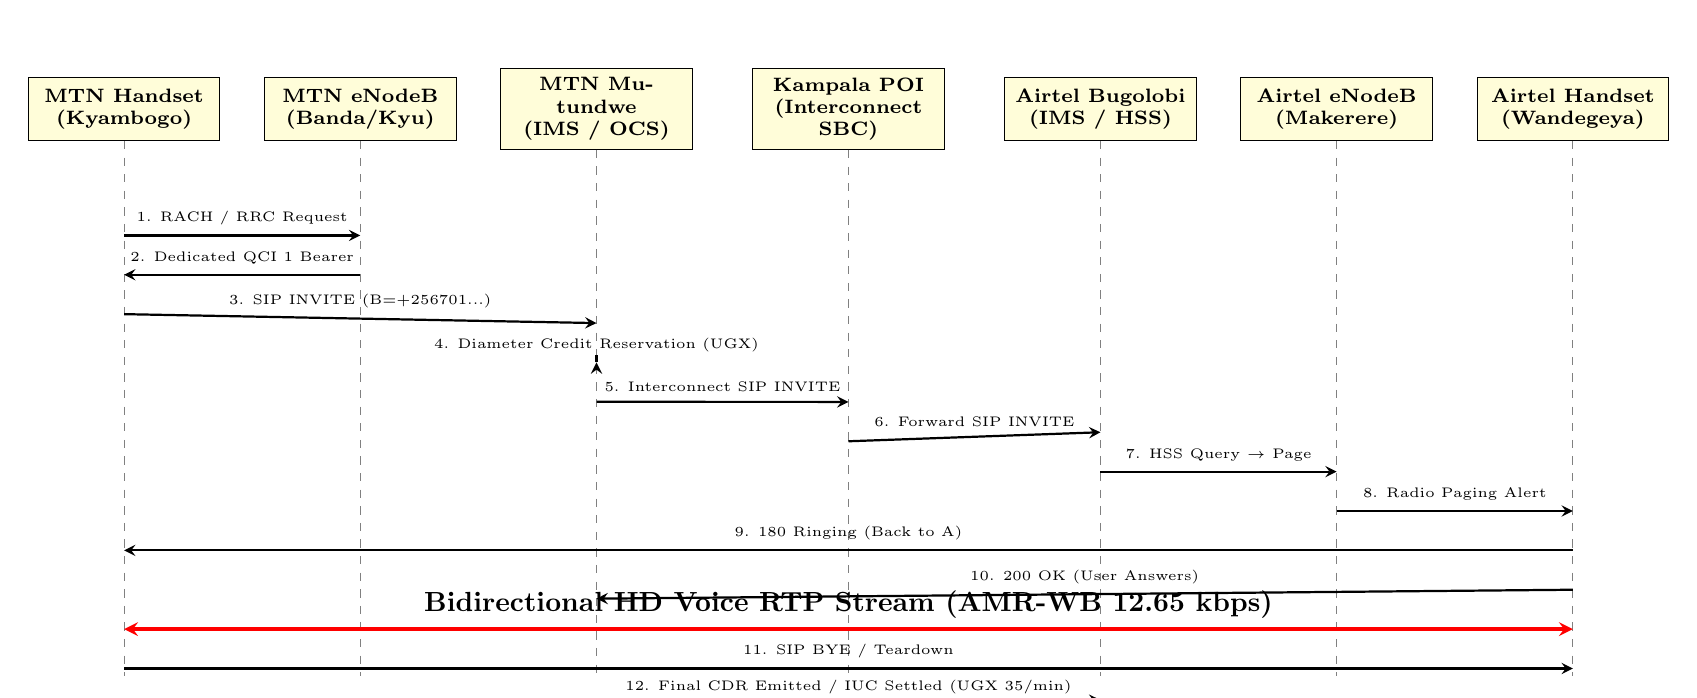
\begin{tikzpicture}[node distance=1.8cm, auto, >=stealth]
\tikzstyle{actor} = [draw, rectangle, fill=yellow!15, text width=2.2cm, text centered, minimum height=0.8cm, font=\scriptsize\bfseries]
\tikzstyle{flow} = [draw, ->, thick, font=\tiny]

% Nodes across the top
\node [actor] (UE_A) {MTN Handset\\(Kyambogo)};
\node [actor, right of=UE_A, xshift=1.2cm] (RAN_A) {MTN eNodeB\\(Banda/Kyu)};
\node [actor, right of=RAN_A, xshift=1.2cm] (CORE_A) {MTN Mutundwe\\(IMS / OCS)};
\node [actor, right of=CORE_A, xshift=1.4cm] (POI) {Kampala POI\\(Interconnect SBC)};
\node [actor, right of=POI, xshift=1.4cm] (CORE_B) {Airtel Bugolobi\\(IMS / HSS)};
\node [actor, right of=CORE_B, xshift=1.2cm] (RAN_B) {Airtel eNodeB\\(Makerere)};
\node [actor, right of=RAN_B, xshift=1.2cm] (UE_B) {Airtel Handset\\(Wandegeya)};

% Vertical life lines
\draw [dashed, gray] (UE_A) -- ++(0,-7.2);
\draw [dashed, gray] (RAN_A) -- ++(0,-7.2);
\draw [dashed, gray] (CORE_A) -- ++(0,-7.2);
\draw [dashed, gray] (POI) -- ++(0,-7.2);
\draw [dashed, gray] (CORE_B) -- ++(0,-7.2);
\draw [dashed, gray] (RAN_B) -- ++(0,-7.2);
\draw [dashed, gray] (UE_B) -- ++(0,-7.2);

% Sequence Messages
\draw [flow] ([yshift=-1.2cm]UE_A.south) -- node[above]{1. RACH / RRC Request} ([yshift=-1.2cm]RAN_A.south);
\draw [flow] ([yshift=-1.7cm]RAN_A.south) -- node[above]{2. Dedicated QCI 1 Bearer} ([yshift=-1.7cm]UE_A.south);
\draw [flow] ([yshift=-2.2cm]UE_A.south) -- node[above]{3. SIP INVITE (B=+256701...)} ([yshift=-2.2cm]CORE_A.south);
\draw [flow] ([yshift=-2.7cm]CORE_A.south) -- node[above]{4. Diameter Credit Reservation (UGX)} ([yshift=-2.7cm]CORE_A.south);
\draw [flow] ([yshift=-3.2cm]CORE_A.south) -- node[above]{5. Interconnect SIP INVITE} ([yshift=-3.2cm]POI.south);
\draw [flow] ([yshift=-3.7cm]POI.south) -- node[above]{6. Forward SIP INVITE} ([yshift=-3.7cm]CORE_B.south);
\draw [flow] ([yshift=-4.2cm]CORE_B.south) -- node[above]{7. HSS Query $\rightarrow$ Page} ([yshift=-4.2cm]RAN_B.south);
\draw [flow] ([yshift=-4.7cm]RAN_B.south) -- node[above]{8. Radio Paging Alert} ([yshift=-4.7cm]UE_B.south);
\draw [flow] ([yshift=-5.2cm]UE_B.south) -- node[above]{9. 180 Ringing (Back to A)} ([yshift=-5.2cm]UE_A.south);
\draw [flow] ([yshift=-5.7cm]UE_B.south) -- node[above]{10. 200 OK (User Answers)} ([yshift=-5.7cm]CORE_A.south);
\draw [<->, very thick, red] ([yshift=-6.2cm]UE_A.south) -- node[above, black]{\textbf{Bidirectional HD Voice RTP Stream (AMR-WB 12.65 kbps)}} ([yshift=-6.2cm]UE_B.south);
\draw [flow] ([yshift=-6.7cm]UE_A.south) -- node[above]{11. SIP BYE / Teardown} ([yshift=-6.7cm]UE_B.south);
\draw [flow] ([yshift=-7.1cm]CORE_A.south) -- node[above]{12. Final CDR Emitted / IUC Settled (UGX 35/min)} ([yshift=-7.1cm]CORE_B.south);

\end{tikzpicture}%
}
\caption{End-to-End Inter-Carrier Call Flow: MTN Uganda to Airtel Uganda}
\label{fig:uganda_interconnect_flow}
\end{figure}

\subsection{Phase-by-Phase Technical Explanation of the Ugandan Interconnect Call}
The technical operations executing across both carriers' infrastructure proceed through distinct, tightly coordinated phases:

\begin{enumerate}
    \item \textbf{Radio Access Connection at Kyambogo University:}
    The MTN subscriber handset transmits a Random Access Channel (RACH) preamble to the serving MTN LTE/5G base station (eNodeB / gNodeB located near Kyambogo University campus). Upon receiving the Random Access Response (RAR), the handset completes Radio Resource Control (RRC) connection setup. For VoLTE, the network establishes a dedicated high-priority Evolved Packet System (EPS) bearer assigned Quality of Service Class Identifier 1 (\textbf{QCI 1}). QCI 1 enforces a maximum packet delay budget of $100\text{ ms}$ and an ultra-low packet error loss rate of $10^{-2}$, guaranteeing crystal-clear speech without packet starvation even when background 4G data downloads are saturated.

    \item \textbf{Originating IMS Core Signaling (Mutundwe):}
    The handset generates a SIP `INVITE` request over the established QCI 1 bearer addressed to the destination SIP URI `sip:+256701654321@mtn.co.ug;user=phone`. This message hits the Proxy-Call Session Control Function (P-CSCF) at MTN's Mutundwe Data Center. The P-CSCF validates the IPsec security association of the handset and forwards the message to the Serving-CSCF (S-CSCF).

    \item \textbf{Pre-Call Real-Time Rating via MTN Online Charging System (OCS):}
    Unlike post-paid corporate accounts in developed nations, over $98\%$ of Ugandan mobile subscribers operate on a prepaid basis. Therefore, before the S-CSCF allows the call to advance beyond the core, it triggers a real-time Diameter Credit-Control Application (DCCA / RFC 4006) request over the \textbf{Diameter Ro} interface to the MTN \textbf{Online Charging System (OCS)} (Huawei CBS platform):
    \begin{itemize}
        \item The OCS checks the caller's main airtime account balance (in Ugandan Shillings - UGX) and voice bundle balance (such as an MTN \textit{Pulse} or \textit{Voice Bundle}).
        \item Under UCC tariff filings, the standard off-net voice tariff applies (e.g., UGX 4.5 per second).
        \item The OCS executes an atomic credit reservation, locking a 60-second quota. If the caller has insufficient funds ($<\text{UGX } 100$), the OCS returns a Diameter rating error (\texttt{DIAMETER\_CREDIT\_LIMIT\_REACHED}), and the S-CSCF redirects the call to an IVR announcement: \textit{``You do not have enough airtime to make this call. Please recharge using MTN MoMo *165\#''.}
    \end{itemize}

    \item \textbf{Number Analysis and Mobile Number Portability (MNP):}
    Once credit is reserved, the S-CSCF performs digit translation on `+256 701 654 321`. The leading national destination code `070` is matched against the UCC numbering allocation table, identifying \textbf{Airtel Uganda} as the recipient carrier. The switch executes a query against the centralized Ugandan Mobile Number Portability (MNP) clearinghouse to verify that the recipient has not ported the number to another network.

    \item \textbf{Point of Interconnect (POI) Transit across Kampala Metro Fiber:}
    The call is directed to MTN's Interconnect Session Border Controller (SBC) at Mutundwe. The SBC enforces carrier topology hiding, rate limiting, and Distributed Denial of Service (DDoS) mitigation. The SBC transmits the SIP `INVITE` across a direct, dual-homed, carrier-grade optical fiber link traversing the Kampala metropolitan ring to Airtel's Interconnect SBC located at Airtel's \textbf{Bugolobi Data Center}.

    \item \textbf{Airtel Core Ingress and Location Interrogation (Bugolobi):}
    Airtel's Interconnect SBC admits the SIP `INVITE` and routes it to Airtel's Interrogating-CSCF (I-CSCF). The I-CSCF issues a Diameter `User-Data-Request` (UDR) to Airtel's \textbf{Home Subscriber Server (HSS)} / Unified Data Management (UDM) database to determine the whereabouts of subscriber `+256 701 654 321`. The HSS responds with the current serving Mobility Management Entity (MME) and cell sector, revealing that the subscriber is currently registered on the Airtel eNodeB tower covering Makerere University and Wandegeya.

    \item \textbf{Paging and Radio Alerting in Wandegeya:}
    Airtel's serving MME sends an S1-AP Paging message to the eNodeB in Wandegeya. The base station transmits a paging message across the radio paging control channel. The recipient handset receives the page, attaches its radio bearer, and rings. Airtel transmits a SIP `180 Ringing` message back across the POI fiber ring to MTN Mutundwe, which forwards it to the Kyambogo handset, causing the caller to hear the standard audible ringback tone.

    \item \textbf{Call Answer, Codec Negotiation, and Conversation:}
    The Airtel subscriber swipes to answer the call. The handset dispatches a SIP `200 OK` message containing its Session Description Protocol (SDP) answer. During this exchange, both networks negotiate the speech codec. By leveraging Transcoder-Free Operation (TrFO), both networks agree on the \textbf{AMR-WB (Adaptive Multi-Rate Wideband)} codec operating at $12.65\text{ kbps}$ (HD Voice). High-fidelity, digitized voice is packetized into Real-time Transport Protocol (RTP) packets transmitted directly between the respective media gateways over the optical interconnect, bypassing unnecessary analog or G.711 transcoding.

    \item \textbf{Active In-Call Rating and Call Teardown:}
    While conversation proceeds, MTN's OCS tracks call duration in real time, debiting the reserved credit balance every 10 seconds. If the user's airtime is depleted during conversation, the OCS drops the session. When the caller terminates the call, the handset sends a SIP `BYE` request. The core tears down the QCI 1 voice bearer and releases radio channel resources.

    \item \textbf{Offline Billing Mediation and Inter-Carrier Settlement (CDR \& IUC):}
    Both operators log the transaction:
    \begin{itemize}
        \item MTN's core generates an originating Call Detail Record (CDR) logging start time, end time, total billable seconds ($T$), caller MSISDN, dialed MSISDN, and outgoing trunk group ID.
        \item Airtel's core generates a terminating CDR logging identical transaction parameters.
        \item \textbf{Interconnect Usage Charge (IUC) Settlement:} Under UCC Interconnection Regulations, MTN collects airtime from its caller and must pay an agreed termination fee to Airtel for utilizing Airtel's radio network to deliver the call. If the call lasted 3 minutes (180 seconds) and the UCC regulated termination rate is $\text{UGX } 35.00/\text{min}$, MTN settles:
        \[ \text{Settlement Payable to Airtel} = 3 \times \text{UGX } 35.00 = \text{UGX } 105.00 \]
        At the end of each calendar month, MTN and Airtel billing clearinghouses perform automated CDR reconciliation, settling the net difference in inter-carrier traffic balances.
    \end{itemize}
\end{enumerate}

\chapter{Switching, Routing, and Trunks}

\section{Routing Principles: Softswitches and Cloud Cores}
Routing in telecommunications is the computational process of selecting an optimal transmission path across interconnected networks to deliver a call to its destination. The Softswitch (or Call Session Control Function in IMS) acts as the intelligent control plane, decoupled from the underlying physical transport media gateways.

\subsection{Five Stages of Telephony Routing}
\begin{enumerate}
    \item \textbf{Digit Analysis:} The switch strips incoming carrier prefixes (e.g., country code $+256$ or domestic access trunk digit $0$) and performs longest-prefix matching against its routing table.
    \item \textbf{Number Translation \& Normalization:} Translating short codes (e.g., dialing $100$ is translated to internal customer support call center hunt groups; dialing emergency $112$ is mapped to national police dispatch).
    \item \textbf{Route Selection and Trunk Group Hunting:} Selecting the primary outbound trunk group with lowest latency and minimum cost.
    \item \textbf{Load Balancing and Proportional Distribution:} Splitting traffic across redundant transmission links (e.g., distributing traffic $50/50$ across East and West fiber rings).
    \item \textbf{Automatic Alternative Routing (AAR / Overflow):} If all circuits on the primary direct trunk group are saturated, the switch automatically diverts overflow traffic across secondary transit trunks without dropping the call.
\end{enumerate}

\section{Trunks, Wires, and Channels}
\begin{itemize}
    \item \textbf{Subscriber Line (Local Loop):} Dedicated physical connection terminating on a single customer handset. In legacy copper, this is a 2-wire unshielded twisted pair carrying $-48\text{V DC}$ battery voltage, analog voice frequencies ($300\text{--}3400\text{ Hz}$), and $75\text{V AC}$ ringing.
    \item \textbf{Trunk:} A shared high-speed multiplexed transmission circuit connecting switching exchanges. A trunk carries multiple concurrent calls simultaneously:
    \[ 1\text{ Voice Channel} = 1\text{ Active Concurrent Call} \]
    \item \textbf{The ITU-T E1 Digital Carrier Standard:} The foundational digital trunk hierarchy in Uganda and Europe. Operating at an aggregate line rate of $2.048\text{ Mbps}$, an E1 frame multiplexes 32 separate $64\text{ kbps}$ time slots (TS):
    \begin{itemize}
        \item \textbf{Time Slot 0 (TS0):} Dedicated to frame synchronization, alignment, and Cyclic Redundancy Check (CRC-4) error detection.
        \item \textbf{Time Slots 1 to 15 and 17 to 31 (30 Channels):} Dedicated user voice and bearer data channels.
        \item \textbf{Time Slot 16 (TS16):} Dedicated out-of-band signaling channel (carrying Common Channel Signaling like SS7 ISUP or Channel Associated Signaling).
    \end{itemize}
\end{itemize}

\section{The Ugandan National E.164 Numbering Plan}
The Uganda Communications Commission (UCC) establishes and regulates the National Numbering Plan in conformity with ITU-T Recommendation E.164. The international E.164 format for Uganda is structured as:
\[ \underbrace{+256}_{\text{Country Code (CC)}} \; \underbrace{\text{XX}}_{\text{National Destination Code (NDC)}} \; \underbrace{\text{XXX XXX}}_{\text{Subscriber Number (SN)}} \]

Table~\ref{tab:uganda_numbering_plan} details the national prefix allocations, operating carriers, and service descriptions across the Ugandan telephony ecosystem.

\begin{table}[H]
\centering
\small
\renewcommand{\arraystretch}{1.25}
\begin{tabularx}{\textwidth}{|>{\bfseries}p{2.8cm}|>{\raggedright\arraybackslash}p{3.5cm}|>{\raggedright\arraybackslash}p{3.2cm}|>{\raggedright\arraybackslash}X|}
\hline
\textbf{Prefix (NDC)} & \textbf{Assigned Operator} & \textbf{Network Type} & \textbf{Operational Status / Notes} \\ \hline
077, 078 & MTN Uganda & Mobile Cellular & Original nationwide GSM/LTE/5G blocks \\ \hline
076 & MTN Uganda & Mobile Cellular & 10-million block allocated by UCC in 2020 \\ \hline
070, 075 & Airtel Uganda & Mobile Cellular & Primary GSM/LTE/5G subscriber blocks \\ \hline
074 & Airtel Uganda & Mobile Cellular & Formerly Africell block; reassigned to Airtel \\ \hline
071 & Uganda Telecom (UTL) & Mobile Cellular & National public operator cellular network \\ \hline
072 & Lycamobile Uganda & Mobile Cellular & National high-speed data \& voice operator \\ \hline
041 (0414) & UTL / Fixed Carriers & Fixed Geographic & Kampala Metropolitan fixed PSTN lines \\ \hline
043 & UTL & Fixed Geographic & Jinja and Eastern Uganda fixed lines \\ \hline
0485 & UTL & Fixed Geographic & Mbarara and Western Uganda fixed lines \\ \hline
0471 & UTL & Fixed Geographic & Gulu and Northern Uganda fixed lines \\ \hline
031, 039 & MTN Business & Fixed Non-Geographic & Enterprise corporate fixed voice / SIP trunks \\ \hline
0800 & Licensed Carriers & Special / Toll-Free & National toll-free numbers (free for caller) \\ \hline
112, 999 & Emergency Services & Emergency Short Code & Uganda Police, Fire, and Ambulance dispatch \\ \hline
*165\# & MTN Uganda & USSD Financial & MTN Mobile Money (MoMo) financial portal \\ \hline
*185\# & Airtel Uganda & USSD Financial & Airtel Money financial portal \\ \hline
*131\#, *175\# & MTN / Airtel & USSD Self-Care & Airtime balance, bundles, and account self-care \\ \hline
\end{tabularx}
\caption{Ugandan National E.164 Numbering Plan and Prefix Allocations}
\label{tab:uganda_numbering_plan}
\end{table}

\section{Interconnect Trunk Dimensioning: MTN-to-Airtel POI Case Study}
In telecommunications traffic engineering, dimensioning the number of circuits required between switching centers during peak busy hours is performed using the \textbf{Erlang B loss formula}. The Erlang B model assumes Poisson call arrivals, negative exponentially distributed holding times, and that blocked calls are cleared (lost).

\subsection{Erlang B Mathematical Formulation}
The probability of call blocking (Grade of Service, $P_b$ or $B$) on a trunk group comprising $C$ parallel channels offered a traffic intensity of $A$ Erlangs is given by:
\begin{equation}
B(C, A) = \frac{\frac{A^C}{C!}}{\sum_{k=0}^{C} \frac{A^k}{k!}}
\label{eq:erlang_b}
\end{equation}
Where traffic intensity $A$ is defined as the product of the average call arrival rate ($\lambda$ calls/hour) and average call holding duration ($h$ hours):
\[ A = \lambda \times h \]

\subsection{Practical Dimensioning Calculation for Kampala Interconnect}
\textbf{Engineering Scenario:} 
During the evening busy hour ($18:30\text{--}19:30$), subscribers on MTN Uganda make an average of $2,700$ cross-network calls to Airtel Uganda. The average duration of each cross-network conversation is measured as $3.333\text{ minutes}$ ($200\text{ seconds}$). The Uganda Communications Commission (UCC) mandates that the Grade of Service (call blocking probability) across inter-carrier Points of Interconnect must not exceed $1.0\%$ ($B \le 0.01$).

\begin{enumerate}
    \item \textbf{Calculate Offered Traffic ($A$):}
    First convert holding time to hours:
    \[ h = \frac{200\text{ s}}{3600\text{ s/hr}} = \frac{1}{18}\text{ hours} \approx 0.05556\text{ hr} \]
    Compute traffic intensity in Erlangs:
    \[ A = \lambda \times h = 2,700\text{ calls/hr} \times \frac{200}{3600}\text{ hr} = \frac{540,000}{3600} = 150.0\text{ Erlangs} \]

    \item \textbf{Determine Required Voice Channels ($C$):}
    To maintain $B(C, 150) \le 0.01$, telecommunications engineers evaluate the Erlang B formula iteratively or consult standard traffic tables. Evaluating Equation~\eqref{eq:erlang_b} reveals:
    \begin{itemize}
        \item For $C = 160$ channels: $B(160, 150) \approx 0.0245$ ($2.45\%$ blocking, exceeds UCC mandate).
        \item For $C = 166$ channels: $B(166, 150) \approx 0.0112$ ($1.12\%$ blocking).
        \item For $C = 167$ channels: $B(167, 150) \approx 0.0097$ ($0.97\%$ blocking, satisfies $B \le 1.0\%$).
    \end{itemize}
    Therefore, a minimum of \textbf{167 concurrent voice channels} are mathematically required.

    \item \textbf{Physical Transmission Mapping to E1 Carrier Trunks:}
    Since legacy digital interconnects utilize ITU-T E1 circuits, where each E1 trunk delivers exactly 30 user voice time slots:
    \[ N_{\text{E1}} = \left\lceil \frac{C}{30} \right\rceil = \left\lceil \frac{167}{30} \right\rceil = \lceil 5.567 \rceil = 6\text{ E1 Carriers} \]
    Provisioning 6 E1 circuits provides $6 \times 30 = 180$ voice channels. With 180 channels, the actual operational blocking drops to $B(180, 150) \approx 0.00067$ ($0.067\%$), providing ample headroom for unexpected traffic spikes during national holidays or mobile marketing campaigns.

    \item \textbf{Modern Optical SIP Session Trunk Mapping:}
    In modern all-IP interconnects between MTN Mutundwe and Airtel Bugolobi, these 167 channels are provisioned as \textbf{167 concurrent SIP sessions} over redundant $10\text{ Gbps}$ optical Ethernet interfaces on the Session Border Controllers (SBCs), with licensed SBC codec transcoding and media policing.
\end{enumerate}

\chapter{Analog vs Digital Transmission}

\section{The Transition to Digital}
\subsection{Analog Transmission}
Analog telephony operates on the principle of continuous electrical waves directly proportional to acoustic sound pressure waves. While conceptually simple, analog transmission suffers from severe fundamental weaknesses:
\begin{itemize}
    \item \textbf{Cumulative Noise Amplification:} Analog amplifiers amplify both the desired voice signal and transmission line thermal noise, degrading signal-to-noise ratio over long distances.
    \item \textbf{Distance Attenuation:} High frequencies experience greater attenuation than low frequencies, causing audio muffling.
    \item \textbf{Inflexibility for Bulk Multiplexing:} Analog frequency-division multiplexing requires costly, bulky analog filters.
\end{itemize}

\subsection{Pulse Code Modulation (PCM)}
To overcome analog limitations, voice is digitized using Pulse Code Modulation (standardized in ITU-T G.711). The human voice contains intelligible frequencies up to $3.4\text{ kHz}$. Digitization executes in three sequential stages:
\begin{enumerate}
    \item \textbf{Sampling (Nyquist Theorem):} The analog signal is sampled at twice the highest voice frequency component ($2 \times 4\text{ kHz}$ to account for filter roll-off), yielding an exact sampling rate of:
    \[ f_s = 8,000\text{ samples per second} \quad (\text{Sampling interval } T_s = 125\,\mu\text{s}) \]
    
    \item \textbf{Quantization and Companding:} Each continuous sample amplitude is mapped to a discrete quantized level using 8-bit logarithmic companding (compressing-expanding):
    \begin{itemize}
        \item \textbf{A-law Companding:} Standardized across Uganda, Africa, and Europe, providing superior dynamic range for low-level signals ($A = 87.6$).
        \item \textbf{$\mu$-law Companding:} Standardized across North America and Japan ($\mu = 255$).
    \end{itemize}
    8 bits yields $2^8 = 256$ discrete quantization levels.
    
    \item \textbf{Encoding:} The quantized level is converted into an 8-bit binary word. The fundamental transmission bit rate for a single toll-quality digital telephone voice channel is:
    \[ \text{Bit Rate} = 8,000\text{ samples/s} \times 8\text{ bits/sample} = 64\text{ kbps} \quad (\text{DS0 standard}) \]
\end{enumerate}

\section{Dial-Up Modems and Character Framing}
Because legacy PSTN networks were engineered strictly for $300\text{--}3400\text{ Hz}$ acoustic audio, computer data could not be transmitted as raw square-wave pulses. A \textbf{modem} (modulator-demodulator) converts binary ones and zeros into audible phase- and frequency-modulated tones.

In asynchronous dial-up communications, characters are framed using the American Standard Code for Information Interchange (ASCII):
\begin{itemize}
    \item 1 Start Bit (transitions line from idle mark to space)
    \item 8 Data Bits (ASCII character payload, LSB first)
    \item 1 Stop Bit (returns line to idle mark state)
    \item \textbf{Total Frame Overhead:} $1 + 8 + 1 = 10\text{ bits per character transmitted}$.
\end{itemize}

\chapter{Data Switching Strategies}

\section{Circuit, Message, and Packet Switching}
Telecommunications data networks deploy three primary switching philosophies to transport information between endpoints:
\begin{enumerate}
    \item \textbf{Circuit Switching:} Dedicated physical or virtual path established prior to communication. Ideal for real-time voice due to constant delay, but bandwidth is wasted during conversational pauses.
    \item \textbf{Message Switching:} The entire message is stored and forwarded from node to node. High delay; obsolete in modern real-time voice telephony.
    \item \textbf{Packet Switching:} Data streams are chopped into discrete, standardized packets containing headers and payloads. Links are dynamically shared using statistical multiplexing. Modern Voice over IP (VoIP), VoLTE, and VoNR operate exclusively on packet-switched IP networks.
\end{enumerate}

\begin{table}[H]
\centering
\small
\renewcommand{\arraystretch}{1.3}
\begin{tabularx}{\textwidth}{|>{\bfseries}p{3.2cm}|>{\raggedright\arraybackslash}X|>{\raggedright\arraybackslash}X|>{\raggedright\arraybackslash}X|}
\hline
\textbf{Feature} & \textbf{Circuit Switching} & \textbf{Message Switching} & \textbf{Packet Switching} \\ \hline
\textbf{Dedicated Path} & Yes, reserved end-to-end & No, store-and-forward & No, dynamically routed \\ \hline
\textbf{Call Setup Phase} & Mandatory setup delay & None required & Connectionless or virtual \\ \hline
\textbf{Transmission Delay} & Minimal, constant & Very high (store-and-forward) & Low to moderate (pipelined) \\ \hline
\textbf{Bandwidth Efficiency} & Low (idle during silence) & Moderate & High (statistical multiplexing) \\ \hline
\textbf{Congestion Behavior} & Call blocked at setup & Delayed in intermediate queues & Jitter / packet drop \\ \hline
\textbf{Primary Telephony Use} & Legacy PSTN, 2G/3G CS & Telegrams, store-and-forward & VoIP, VoLTE, VoNR, 5G Core \\ \hline
\end{tabularx}
\caption{Comprehensive Comparison of Telecommunications Switching Strategies}
\label{tab:switching_comparison}
\end{table}

\chapter{Telephony Data Systems (OSS/BSS)}

\section{The Functional Separation: OSS versus BSS}
In carrier-grade telecommunications, data systems are divided into two interdependent computational architectures:
\begin{itemize}
    \item \textbf{Operations Support Systems (OSS):} The network-facing computational plane. OSS platforms interact directly with physical switches, routers, base stations, and transmission equipment to monitor infrastructure health, automate service provisioning, configure network elements, and orchestrate maintenance.
    \item \textbf{Business Support Systems (BSS):} The customer- and commerce-facing computational plane. BSS platforms administer subscriber accounts, product catalogs, customer relationship management (CRM), convergent rating and billing, revenue assurance, and fraud prevention.
\end{itemize}

\section{The ISO FCAPS Management Framework}
Carrier Network Operations Centers (NOCs) utilize the ISO FCAPS structural model to categorize network management operations:
\begin{itemize}
    \item \textbf{Fault Management (F):} Real-time detection, filtering, correlation, and automated ticketing of network alarms (e.g., loss of signal, laser degradation, power failure).
    \item \textbf{Configuration Management (C):} Maintaining hardware and software inventories, automating firmware rollouts, managing network device backups, and provisioning new subscriber SIMs.
    \item \textbf{Accounting Management (A):} Ingesting, mediating, and formatting Call Detail Records (CDRs) and data IP detail records (IPDRs) for billing and inter-carrier settlement.
    \item \textbf{Performance Management (P):} Continuous statistical tracking of network Key Performance Indicators (KPIs), including Busy Hour Call Attempts (BHCA), Answer-Seizure Ratio (ASR), packet loss, and Erlang traffic load.
    \item \textbf{Security Management (S):} Enforcing Role-Based Access Control (RBAC), multi-factor authentication for switch administration, optical link encryption, and real-time telecom fraud detection (such as SIM boxing and international revenue share fraud).
\end{itemize}

\section{OSS and BSS Architectures in Ugandan MNOs (MTN and Airtel)}
The operational reality of telecommunications in Uganda has shaped distinct, highly specialized OSS and BSS deployments tailored to high-volume micro-transactions, extensive prepaid usage, and widespread mobile financial services.

\subsection{Ugandan BSS Ecosystem: Prepaid Rating and Mobile Fintech}
\begin{itemize}
    \item \textbf{Convergent Real-Time Online Charging Systems (OCS):}
    Because more than $98\%$ of consumers in Uganda use prepaid SIM cards, billing cannot occur retroactively at the end of the month. MTN Uganda deploys the \textbf{Huawei Convergent Billing System (CBS)}, while Airtel Uganda runs the \textbf{Ericsson Charging System (ECS)}. These platforms process millions of real-time transactions per second using the Diameter Credit-Control protocol (over 3GPP Gy and Ro interfaces). When an MTN or Airtel subscriber dials a call, streams a YouTube video, or sends an SMS, the OCS decrements airtime or bundle units in sub-second cycles.
    
    \item \textbf{The Convergence of Telecom and Mobile Money (MoMo and Airtel Money):}
    Uganda is recognized globally as a pioneer in mobile financial services. Under the National Payment Systems (NPS) Act 2020 administered by the Bank of Uganda, \textbf{MTN Mobile Money Uganda Limited} and \textbf{Airtel Mobile Commerce Uganda Limited} operate as licensed, independent Payment System Operators (PSOs) legally ring-fenced from their parent telecom entities.
    \begin{itemize}
        \item \textit{Architectural Integration:} The mobile money core interacts directly with the cellular network via high-throughput \textbf{Unstructured Supplementary Service Data (USSD)} gateways (`*165\#' for MTN, `*185\#' for Airtel) and mobile applications over encrypted HTTPS REST APIs.
        \item \textit{Prepaid Bundle Fulfillment:} Over $70\%$ of voice and data bundles in Uganda are purchased directly through mobile money wallets rather than physical scratch cards. When a subscriber dials `*165*2\#' to purchase an MTN voice bundle, the MoMo transactional switch verifies PIN authentication, debits the user's electronic wallet ledger, issues an ISO 8583 banking credit confirmation, and triggers a Diameter API call to the telecom BSS OCS to immediately credit the subscriber's voice quota.
    \end{itemize}
\end{itemize}

\subsection{Ugandan OSS Ecosystem: 24/7 NOCs and Towerco Telemetry}
\begin{itemize}
    \item \textbf{Centralized Network Operations Centers (NOC):}
    MTN operates its primary national Tier-1/Tier-2/Tier-3 Network Operations Center at the \textbf{Mutundwe Data Center} in Kampala, while Airtel runs its central NOC from its \textbf{Bugolobi Facility}. These control rooms feature massive monitoring video walls running vendor NMS platforms: \textbf{Huawei iManager Mobile Automation Engine (MAE) / U2000} and \textbf{Ericsson Network Manager (ENM)}. Engineers monitor real-time heat maps, cell site outages, fiber link status, and UCC QoS telemetry across Uganda 24 hours a day, 365 days a year.
    
    \item \textbf{Passive Infrastructure Management via Towercos (ATC Uganda):}
    Because cellular towers across Uganda are largely owned and managed by \textbf{American Tower Corporation (ATC Uganda)}, the OSS interface bridges between the mobile operator and the tower company. ATC equips thousands of remote tower sites with IoT supervisory controllers (such as Netbiter or Huawei NetEco units). These sensors stream telemetry over cellular 4G IoT links to report:
    \begin{itemize}
        \item Commercial UMEME electrical grid voltage and phase failure.
        \item Diesel generator running hours, fuel tank depth sensors (to detect fuel theft), and oil temperature.
        \item Hybrid solar photovoltaic MPPT charger current and $48\text{V}$ lithium/lead-acid battery string voltages.
        \item Tower compound security fence breach and shelter temperature alarms.
    \end{itemize}
    When a power fault occurs at a remote site in Kitgum or Kisoro, ATC's automated OSS correlates the telemetry and dispatches local rapid-response maintenance crews with mobile diesel generators before battery backup drains below the $-44\text{V DC}$ low-voltage threshold.
\end{itemize}

\chapter{Maintenance Strategies}

\section{Four Core Types of Maintenance and System Reliability}
In modern telecommunications data systems, maintenance is the operational discipline that preserves network availability, signal fidelity, and customer quality-of-service (QoS). Telecommunications infrastructure comprises both physical outside plant (cables, poles, cabinets) and logical systems (switches, databases, signaling links). Maintenance strategies are categorized into four distinct methodologies based on their operational triggers, costs, and downtime implications:

\subsection{Corrective Maintenance (Reactive / Unplanned)}
Corrective maintenance comprises actions performed strictly after a functional failure, circuit outage, or physical fault has occurred. The primary objective is to restore the service to operational status as rapidly as possible. While corrective maintenance requires minimal routine scheduling overhead, it causes unpredictable network downtime, severe Service Level Agreement (SLA) financial penalties, and catastrophic customer dissatisfaction.
\begin{itemize}
    \item \textbf{Characteristics:} High Mean Time to Repair (MTTR), emergency technician call-outs, expedited component replacement costs, and unplanned network re-routing.
    \item \textbf{Ugandan Industry Example (Civil Roadworks Fiber Cuts):} In Uganda, one of the most frequent operational triggers for corrective maintenance is accidental fiber severance caused by road construction and civil works by the Uganda National Roads Authority (UNRA) or municipal trenching along corridors such as the Kampala--Jinja Highway, Entebbe Expressway, and the Northern Bypass. When an excavator severs MTN Uganda's 96-core underground metro fiber ring near Banda or Bweyogerere, thousands of mobile and enterprise data users are immediately disconnected. MTN's Network Operations Center (NOC) at Mutundwe immediately dispatches emergency outside-plant (OSP) splicing teams equipped with Optical Time-Domain Reflectometers (OTDRs) and precision fusion splicers to locate the physical break, pull slack cable, and fuse the fibers inside a waterproof joint closure.
    \item \textbf{Ugandan Industry Example (Rural BTS Power Outages):} Similarly, Airtel Uganda frequently executes urgent corrective maintenance across remote off-grid Base Transceiver Stations (BTS) in rural areas (such as Karamoja, West Nile, or Kisoro) when commercial power grid outages from UMEME coincide with backup diesel generator starter motor failures, requiring emergency field technicians to service fuel injectors or replace depleted batteries before the $-48\text{V DC}$ system drops below the $-44\text{V DC}$ Low Voltage Disconnect (LVD) threshold.
\end{itemize}

\subsection{Preventive Maintenance (Time-Scheduled / Routine)}
Preventive maintenance consists of predetermined, time-scheduled inspections, cleaning, testing, and component servicing conducted at fixed calendar intervals regardless of current operating status. Its primary objective is to reduce the probability of hardware failure by detecting gradual wear, environmental degradation, and resource depletion before an outage occurs.
\begin{itemize}
    \item \textbf{Characteristics:} Predictable operational expenditure (OPEX), scheduled maintenance windows (typically during low-traffic periods between 01:00 and 05:00), and prolonged equipment lifespan.
    \item \textbf{Ugandan Industry Example (Hybrid Solar-Diesel Tower Sites):} Due to commercial grid unreliability across rural Uganda, both MTN Uganda and Airtel Uganda rely on hybrid power architectures (often managed in partnership with tower infrastructure providers such as ATC Uganda). Preventive maintenance schedules dictate monthly generator servicing (oil, air filter, and fuel filter replacement every 250 operational hours) and quarterly conductance and capacity testing on $48\text{V}$ Valve-Regulated Lead-Acid (VRLA) or Lithium Iron Phosphate ($\text{LiFePO}_4$) battery banks to prevent catastrophic deep-discharge cell failure during grid blackouts.
    \item \textbf{Ugandan Industry Example (Tropical Lightning \& Dust Mitigation):} In regions prone to intense tropical lightning storms (such as the Rwenzori region, Mbale, and Kabale), technicians conduct bi-monthly preventive audits of Telecommunications Grounding Busbars (TGB), testing lightning earth rod resistance with a ground clamp meter to ensure earth resistance remains strictly below $5\,\Omega$ prior to the March--May and September--November rainy seasons. Furthermore, in dusty urban environments like Nakawa and Bugolobi, outdoor BTS cabinet air filters and heat exchangers are cleaned monthly to prevent thermal shutdown of power amplifiers.
\end{itemize}

\subsection{Predictive Maintenance (Condition-Based / Data-Driven)}
Predictive maintenance is an advanced data-driven paradigm that continuously monitors real-time telemetry, operational metrics, and physical parameters to forecast impending failures before any service degradation is experienced by users. Rather than relying on arbitrary calendar intervals, servicing is scheduled only when measured performance indicators cross statistical degradation thresholds.
\begin{itemize}
    \item \textbf{Characteristics:} Maximized component utilization, minimal unnecessary maintenance labor, and near-zero unscheduled downtime.
    \item \textbf{Ugandan Industry Example (MTN DWDM Optical Telemetry):} MTN Uganda operates a national Dense Wavelength Division Multiplexing (DWDM) optical backbone linking Kampala, Masaka, Mbarara, Fort Portal, Gulu, and Mbale. Telemetry systems continuously track the Optical Signal-to-Noise Ratio (OSNR) and pre-Forward Error Correction (pre-FEC) Bit Error Rate on 100 Gbps and 200 Gbps coherent transponders. If the pre-FEC BER on the Kampala--Mbarara fiber span crosses $10^{-5}$ due to fiber bend strain or connector contamination, automated NMS ticketing alerts optical transport engineers to clean LC connectors and re-tune optical attenuators during scheduled night maintenance windows before uncorrectable frame loss disrupts subscriber data.
    \item \textbf{Ugandan Industry Example (Airtel Tower Feeder VSWR Monitoring):} Similarly, Airtel Uganda continuously polls the Voltage Standing Wave Ratio (VSWR) on coaxial jumpers connecting tower-mounted Remote Radio Units (RRUs) to sectoral antennas across major cell sites (e.g., Kololo, Naguru, and Tank Hill in Kampala). A gradual upward drift in VSWR from 1.15 to 1.35 indicates weatherproofing tape degradation and tropical rainwater ingress into the RF connector, prompting antenna riggers to reseal the jumper before reflected RF power causes power amplifier burnout.
\end{itemize}

\subsection{Adaptive Maintenance (Evolutionary / Improvement)}
Adaptive maintenance involves modifications, firmware updates, software patches, and hardware alterations undertaken to adapt the operational telecommunications system to evolving business requirements, new protocols, updated regulatory mandates, or changing traffic demands.
\begin{itemize}
    \item \textbf{Characteristics:} Planned architectural evolution, backward compatibility testing, and protocol interoperability verification.
    \item \textbf{Ugandan Industry Example (NIRA Biometric SIM Integration):} Both MTN Uganda and Airtel Uganda carried out major adaptive software and network enhancements to comply with Uganda Communications Commission (UCC) directives requiring real-time biometric SIM card registration. Engineers developed secure API bridges connecting their Home Subscriber Servers (HSS), Unified Data Management (UDM) databases, and Mobile Money (MTN MoMo and Airtel Money) charging gateways directly with the National Identification and Registration Authority (NIRA) database for real-time biometric National Identification Number (NIN) verification.
    \item \textbf{Ugandan Industry Example (Spectrum Re-farming):} Furthermore, both operators continuously conduct spectrum re-farming---reallocating legacy 900 MHz and 1800 MHz 2G GSM frequencies into high-capacity 4G LTE and 5G NR carrier bands to accommodate surging mobile data consumption across Ugandan universities and urban centers.
\end{itemize}

\subsection{System Reliability and Availability Modeling}
The mathematical effectiveness of a maintenance strategy is quantified through system availability ($A$), defined as:
\[ A = \frac{\text{MTBF}}{\text{MTBF} + \text{MTTR}} \]
Where:
\begin{itemize}
    \item \textbf{MTBF (Mean Time Between Failures):} The average operational runtime elapsed between inherent system failures during normal operational conditions.
    \item \textbf{MTTR (Mean Time To Repair):} The average duration required to troubleshoot, repair or replace, and verify a failed network component back into active service.
\end{itemize}
Telecommunications carriers aim for ``Five Nines'' availability ($99.999\%$), permitting a maximum of only $5.26\text{ minutes}$ of total unscheduled downtime per year across all primary switching and transmission nodes. Achieving five nines requires minimizing MTTR through modular hot-swappable line cards, automated failover trunks, and predictive telemetry.

\section{The Cisco Six-Step Troubleshooting Methodology}
Telecommunications field engineers and Network Operations Center (NOC) teams follow the structured Cisco six-step diagnostic framework to systematically isolate and resolve network anomalies without introducing secondary faults:

\begin{enumerate}
    \item \textbf{Identify the Problem:} Gather factual symptoms from customer fault tickets, automated NMS traps, and monitoring alerts. Establish the precise nature of the failure, timestamp of onset, affected geographic areas, and blast radius (whether localized to a single subscriber loop or impacting an entire exchange trunk group).
    
    \item \textbf{Theorize the Probable Cause:} Review recent change management logs, firmware upgrades, and physical plant maintenance activities. Apply the OSI reference model (using Bottom-Up, Top-Down, or Divide-and-Conquer diagnostic approaches) to formulate a prioritized list of plausible hypotheses grounded in engineering principles.
    
    \item \textbf{Test the Theory:} Systematically evaluate hypotheses starting from the most likely cause. Isolate variables by testing one parameter at a time. Utilize diagnostic command-line tools (\texttt{ping}, \texttt{traceroute}, \texttt{show interfaces}) or hardware test sets (optical power meters, OTDRs, digital multimeters) to confirm or refute each hypothesis.
    
    \item \textbf{Establish and Implement a Plan of Action:} Formulate a detailed remediation plan including rollback procedures. Obtain change-window authorization if required, and implement the necessary configuration change, hardware replacement, or software patch cleanly.
    
    \item \textbf{Verify Full System Functionality:} Conduct end-to-end verification testing to confirm that the reported fault is eliminated and that associated telemetry metrics (latency, packet loss, jitter, BER, Answer-Seizure Ratio) satisfy defined Service Level Agreements (SLAs).
    
    \item \textbf{Document Findings, Actions, and Outcomes:} Formulate a detailed Post-Incident Review (PIR). Record the root cause, diagnostic steps, resolution actions, and preventive measures in the central ticketing database to enrich organizational knowledge and expedite future troubleshooting.
\end{enumerate}

\subsection{Practical Ugandan Case Study: Inter-Carrier Trunk Failure (MTN to Airtel Interconnect)}
To illustrate the application of this diagnostic framework in the Ugandan context, consider a real-world scenario involving cross-network call failures between MTN Uganda and Airtel Uganda:
\begin{itemize}
    \item \textbf{Step 1 (Identify the Problem):} During the evening busy hour ($18:30\text{--}20:30$), subscribers on the MTN Uganda network (prefix 077/078) attempting to call Airtel Uganda numbers (prefix 070/075) report immediate call drops and rapid busy signals. In the MTN NOC at Mutundwe, monitoring dashboards display a precipitous drop in the Answer-Seizure Ratio (ASR) on the Point of Interconnect (POI) trunk group from a normal $68\%$ down to $14\%$.
    
    \item \textbf{Step 2 (Theorize Probable Cause):} Engineering teams formulate three technical hypotheses:
    \begin{enumerate}
        \item Physical Layer: Fiber optic severed between MTN Mutundwe Data Center and the Airtel Bugolobi Switching Center.
        \item Signaling Layer: SIP / SS7 signaling link failure or Session Border Controller (SBC) session capacity saturation.
        \item Routing / Database Layer: Corrupted B-number analysis tables in the softswitch failing to recognize newly allocated Airtel numbering blocks (such as the 074 prefix).
    \end{enumerate}
    
    \item \textbf{Step 3 (Test the Theory):} Engineers execute structured diagnostics:
    \begin{itemize}
        \item Physical check: \texttt{show interfaces GigabitEthernet0/0/1} confirms the metro interconnect fiber interface is \texttt{UP/UP} with zero CRC errors, ruling out a physical fiber cut.
        \item Signaling check: Engineers examine SIP error logs on the Session Border Controller and observe an influx of \texttt{SIP 503 Service Unavailable} status codes returned by the destination interconnect gateway. Signaling buffer utilization has reached $100\%$, confirming that concurrent call attempts exceeded the licensed SBC session threshold during a nationwide mobile promotion.
    \end{itemize}
    
    \item \textbf{Step 4 (Implement Plan of Action):} Working in coordination under UCC inter-operator guidelines, engineers from MTN and Airtel activate temporary burst licenses on the Session Border Controllers and dynamically re-allocate 16 additional E1 time slots across secondary inter-carrier routes via the Uganda Telecom (UTL) national transit exchange.
    
    \item \textbf{Step 5 (Verify System Functionality):} Automated test calling robots generate 50 simultaneous cross-network test calls across all prefix combinations. The ASR recovers to $71\%$, voice quality checks confirm Mean Opinion Score (MOS) $\ge 4.1$, and billing mediation validates accurate real-time CDR generation.
    
    \item \textbf{Step 6 (Document Findings):} Both operators log the incident in their respective ITSM platforms, submit a joint regulatory report to the UCC, and initiate a permanent upgrade project to double inter-carrier SIP signaling capacity.
\end{itemize}

\section{Command-Line Interface (CLI) Diagnostic Toolset}
In modern telephony IP backbones and data switching networks, engineers execute specialized CLI diagnostic utilities to inspect control and user planes:
\begin{itemize}
    \item \texttt{ping} \textbf{and Extended Ping:} Injects ICMP Echo Request packets to verify end-to-end Layer 3 reachability. Extended ping allows engineers to manipulate packet size (e.g., sweeping from 64 to 1500 bytes to diagnose buffer issues), set the Don't Fragment (DF) bit to discover Path MTU, and vary the Type of Service (ToS/DSCP) byte to test prioritized voice queuing.
    
    \item \texttt{traceroute} \textbf{/} \texttt{tracert:} Progressively increments the IP packet Time-To-Live (TTL) field starting from $\text{TTL} = 1$ to map the exact intermediate Layer 3 hop-by-hop path, pinpointing transit delay spikes, routing loops, and asymmetric peering paths.
    
    \item \texttt{show interfaces:} Provides comprehensive Layer 1 and Layer 2 operational statistics:
    \begin{itemize}
        \item \textit{Input Errors / CRC Errors:} Indicates physical transmission line noise, faulty cabling, or mismatched clock synchronization on serial/E1 circuits.
        \item \textit{Output Drops:} Signifies interface buffer saturation caused by traffic congestion.
        \item \textit{Duplex / Speed Mismatch:} Detected via late collisions and runt frame counters.
    \end{itemize}
    
    \item \texttt{show ip route} \textbf{\& Protocol Neighbors:} Inspects routing table convergence and protocol adjacency states (e.g., verifying BGP neighbor states transition to \texttt{Established} or OSPF neighbors to \texttt{Full}).
    
    \item \texttt{show logging:} Displays local circular buffer logs categorized by severity level (from Level 0 Emergency to Level 7 Debugging), providing chronological timestamps of link flaps, BGP resets, and environmental threshold alarms.
\end{itemize}

\section{Physical-Layer Transmission Line Testing and Sectionalization}
Physical transmission paths represent the most vulnerable component of telecommunications outside plant. Systematic physical-layer testing isolates faults across copper and fiber infrastructure.

\subsection{Metallic Copper Loop Sectionalization}
In analog and DSL subscriber access networks, high-resistance faults, insulation degradation, and moisture ingress cause severe audio noise, crosstalk, and call drops.
\begin{itemize}
    \item \textbf{Loop Resistance Measurement:} Measures the total loop DC resistance of the pair ($R_{\text{loop}} = 2 \times R_{\text{conductor}}$). For standard 24 AWG ($0.5\text{ mm}$) copper cable, resistance is approximately $84\,\Omega/\text{km}$ loop. If measured resistance deviates significantly from calculated loop distance, a high-resistance splice or corroded terminal is indicated.
    
    \item \textbf{Insulation Resistance (Megger Testing):} Applies a $250\text{V}$ or $500\text{V DC}$ test voltage across Tip-to-Ring, Tip-to-Ground, and Ring-to-Ground. Normal dry paper or plastic insulated cable must demonstrate insulation resistance exceeding $10\,\text{M}\Omega$. Readings below $1\,\text{M}\Omega$ indicate water ingress, pinholes, or sheath damage.
    
    \item \textbf{Sectionalization Workflow:} Field technicians test iteratively across distribution points: Main Distribution Frame (MDF at exchange) $\rightarrow$ Primary Cross-Connection Point (PCP / Street Cabinet) $\rightarrow$ Distribution Point (DP on pole) $\rightarrow$ Network Interface Device (NID at subscriber premises). By sectionalizing the line at each disconnect point, faults are pinpointed to specific cable spans.
\end{itemize}

\subsection{Optical Fiber Transmission Testing}
Optical fiber backbones carry high-density DWDM and E1 trunk aggregates, where minute physical disruptions cause massive data loss.
\begin{itemize}
    \item \textbf{Optical Power Meter \& Light Source (OLTS):} Measures total end-to-end optical insertion loss in decibels ($\text{dB}$) at calibrated wavelengths ($1310\text{ nm}$ and $1550\text{ nm}$):
    \[ \text{Loss (dB)} = P_{\text{transmitted}} (\text{dBm}) - P_{\text{received}} (\text{dBm}) \]
    
    \item \textbf{Optical Time-Domain Reflectometry (OTDR):} Emits high-energy laser light pulses down the fiber core and records the precise timing and amplitude of backscattered light:
    \begin{itemize}
        \item \textit{Rayleigh Backscattering:} Smooth continuous drop along the trace representing uniform fiber attenuation (typically $0.35\text{ dB/km}$ at $1310\text{ nm}$ and $0.20\text{ dB/km}$ at $1550\text{ nm}$).
        \item \textit{Fresnel Reflections:} Sharp upward reflective spikes caused by refractive index discontinuities at mechanical connectors, mechanical splices, or cleaved fiber breaks.
        \item \textit{Macrobend Detection:} A macrobend produces significantly higher attenuation at $1550\text{ nm}$ than at $1310\text{ nm}$, distinguishing physical cable pinching from fusion splices.
    \end{itemize}
\end{itemize}

\section{Telecommunications Diagnostic Baselines, SLA Metrics, and UCC QoS Regulations}
In Uganda, telecommunications service quality is governed by strict regulatory benchmarks enforced by the Uganda Communications Commission (UCC). The UCC conducts quarterly independent drive tests across major highways and urban centers (Kampala, Jinja, Mbarara, Gulu, Fort Portal, and Mbale) to verify that operators comply with Quality of Service (QoS) mandates:
\begin{itemize}
    \item \textbf{Call Setup Success Rate (CSSR):} Mandated to be $\ge 98.0\%$. Measures the percentage of call attempts that successfully establish a voice channel.
    \item \textbf{Call Drop Rate (CDR):} Mandated to be $\le 1.0\%$. Measures the proportion of successfully established calls terminated prematurely due to network fault or radio handover failure.
    \item \textbf{Blocked Call Rate:} Mandated to be $\le 2.0\%$. Quantifies call attempts blocked due to network congestion or insufficient radio channel capacity.
    \item \textbf{Speech Quality (MOS):} Evaluated using the Perceptual Objective Listening Quality Assessment (POLQA) algorithm, requiring a Mean Opinion Score of $\text{MOS} \ge 3.5$.
\end{itemize}

Failure to maintain these thresholds attracts punitive financial sanctions under the Uganda Communications Act. Table~\ref{tab:maintenance_metrics} details the primary diagnostic parameters, baseline acceptable thresholds, failure conditions, and corrective engineering actions across telecommunications systems.

\begin{table}[H]
\centering
\footnotesize
\renewcommand{\arraystretch}{1.3}
\begin{tabularx}{\textwidth}{|>{\raggedright\arraybackslash}p{2.6cm}|>{\raggedright\arraybackslash}p{2.6cm}|>{\raggedright\arraybackslash}p{2.8cm}|>{\raggedright\arraybackslash}X|}
\hline
\textbf{Diagnostic Parameter} & \textbf{Normal Operating Baseline} & \textbf{Failure Threshold} & \textbf{Corrective Maintenance Action} \\ \hline
\textbf{Copper Loop Resistance} & $<1300\,\Omega$ ($24\text{ AWG}$, loop distance dependent) & $>1500\,\Omega$ or $>5\,\Omega$ pair imbalance & Sectionalize cable spans; clean corroded DP terminals; resplice high-resistance joints. \\ \hline
\textbf{Insulation Resistance} & $>10\,\text{M}\Omega$ (Tip-Ring, Tip-Gnd, Ring-Gnd) & $<1\,\text{M}\Omega$ (low insulation / short) & Locate water ingress point; purge cable conduit; replace defective drop wire. \\ \hline
\textbf{Optical Fiber Attenuation} & $0.20\text{ dB/km}$ ($1550\text{ nm}$), $0.35\text{ dB/km}$ ($1310\text{ nm}$) & $>0.50\text{ dB/km}$ or fusion splice $>0.1\text{ dB}$ & Re-clean connector endfaces; re-cleave and re-splice fiber with fusion splicer. \\ \hline
\textbf{Bit Error Rate (BER)} & $<10^{-9}$ (clean digital E1/Ethernet link) & $>10^{-6}$ (degraded), $>10^{-3}$ (sync loss) & Inspect SFP transceivers; verify clock timing; eliminate EMI noise sources. \\ \hline
\textbf{Answer-Seizure Ratio (ASR)} & $60\% - 75\%$ (normal consumer telephony) & $<40\%$ (severe network congestion/fault) & Investigate trunk group capacity; check B-party exchange status; reroute traffic. \\ \hline
\textbf{Exchange DC Power} & $-48\text{V DC}$ (float charge $-54\text{V}$) & $<-44\text{V DC}$ or AC ripple $>100\text{ mV}$ & Replace degraded battery cells; calibrate rectifier modules; check inverter load. \\ \hline
\end{tabularx}
\caption{Telecommunications Diagnostic Baselines, Fault Thresholds, and Corrective Actions}
\label{tab:maintenance_metrics}
\end{table}

\chapter{Emerging Technologies in Telecommunication Data Systems}

\section{Artificial Intelligence for IT Operations (AIOps) and Zero-Touch Telephony}
The unprecedented scale and heterogeneity of modern telecommunications networks have rendered traditional manual Network Operations Center (NOC) monitoring unsustainable. Modern networks ingest millions of performance metrics, event logs, and status traps per second. In response, operators are aggressively deploying \textbf{AIOps (Artificial Intelligence for IT Operations)} to achieve autonomous, ``zero-touch'' network operation.

\subsection{Streaming Telemetry vs. Polling Architectures}
Traditional Network Management Systems (NMS) relied on the Simple Network Management Protocol (SNMP) polling MIB variables over 5- to 15-minute intervals. In high-density carrier backbones, periodic polling introduces unacceptable latency and CPU overhead. AIOps shifts this paradigm to \textbf{model-driven streaming telemetry} (utilizing gRPC, NETCONF/YANG, and Apache Kafka). Network elements continuously push fine-grained operational metrics (sub-second CPU load, interface packet drops, optical transceiver laser currents) to centralized data lakes.

\subsection{Multimodal Anomaly Detection and Alarm Storm Suppression}
When a core fiber trunk is severed, thousands of downstream switches, base stations, and IP routers concurrently lose connectivity, generating a massive ``alarm storm'' of secondary notifications. Human engineers can take hours to sift through thousands of alerts. AIOps platforms utilize unsupervised clustering algorithms, Isolation Forests, and \textbf{Graph Neural Networks (GNNs)} overlaid on real-time network topology maps. The system automatically suppresses redundant cascading alarms, pinpoints the root cause to a specific physical span within milliseconds, and opens a targeted work order for field technicians.

\subsection{Closed-Loop Self-Healing Automata}
Beyond passive diagnostics, AIOps enables closed-loop automated remediation:
\begin{enumerate}
    \item \textbf{Observe:} Ingest real-time telemetry from transport interfaces and call detail records (CDRs).
    \item \textbf{Orient \& Decide:} Machine learning models predict link saturation or circuit degradation before failure occurs.
    \item \textbf{Act:} The cognitive engine automatically orchestrates network changes'''such as rerouting SIP trunk traffic across secondary multi-protocol label switching (MPLS) paths or dynamically spinning up virtual softswitch instances'''without human intervention.
\end{enumerate}

\section{Network Digital Twins (NDT) in Telephony Infrastructure}
A \textbf{Network Digital Twin (NDT)} is a high-fidelity virtual software model that mirrors the physical telecommunications network in real time. By continuously synchronizing physical network states with virtual simulation models, NDTs transform how telecommunication providers plan, test, and optimize infrastructure.

\subsection{Continuous State Synchronization and Modeling}
An NDT integrates three computational layers:
\begin{itemize}
    \item \textbf{Physical Layer:} Core optical backbones, base stations, PBX switches, and subscriber distribution points.
    \item \textbf{Synchronization Pipeline:} High-speed telemetry buses that feed real-time routing tables (BGP, OSPF), link status, traffic volumes, and equipment temperatures into the twin.
    \item \textbf{Simulation \& Analytics Engine:} Computational graph engines that simulate packet flows, electromagnetic wave propagation, and call setup delays.
\end{itemize}

\subsection{Predictive What-If Simulation and Disaster Stress Testing}
Telecom operators utilize Digital Twins to perform non-intrusive ``what-if'' scenario simulations. For example, network architects can simulate the sudden failure of an international undersea fiber gateway or a catastrophic regional power blackout. The Digital Twin simulates resulting traffic rerouting, predicts cascading congestion bottlenecks at transit tandems, and validates whether backup trunk groups have sufficient Erlang capacity to handle redirected busy-hour call volumes.

\subsection{Zero-Risk Staging for Firmware and Configuration Changes}
Human configuration errors represent one of the leading causes of unscheduled network downtime in carrier routing and switching. By staging major software updates, BGP peering policy modifications, or softswitch routing migrations within the virtual Digital Twin first, engineers verify behavior and identify configuration conflicts with zero risk to live subscriber traffic.

\section{Cloud-Native OSS/BSS and Container Orchestration}
The software foundation of telecommunications has completed a paradigm shift away from proprietary, monolithic hardware appliances toward cloud-native microservices architectures.

\subsection{Evolution from Monoliths to Microservices}
Historically, telecommunications switching and billing relied on monolithic hardware systems'''such as Siemens EWSD and Ericsson AXE exchanges'''where software logic was tightly bound to specialized proprietary circuit boards. With the advent of Network Functions Virtualization (NFV), telecom functions moved to Virtual Machines (VMs). Today, the industry has standardized on \textbf{Cloud-Native Network Functions (CNFs)}, where software is decomposed into lightweight, stateless microservices packaged in Open Container Initiative (OCI) containers and orchestrated via \textbf{Kubernetes}.

\subsection{Event-Driven Architecture and Distributed Big Data Pipelines}
Modern Business Support Systems (BSS) require sub-second rating and charging for millions of concurrent data sessions and VoLTE/VoNR voice calls. Cloud-native BSS platforms deploy \textbf{Event-Driven Architectures (EDA)}:
\begin{itemize}
    \item \textbf{Apache Kafka Clusters:} Ingest tens of millions of Call Detail Records (CDRs) and IP data session logs per minute with zero data loss.
    \item \textbf{Distributed Stream Processors (Apache Flink):} Perform real-time rating, credit balance verification, and fraud scoring as calls progress.
    \item \textbf{Polyglot Persistence:} Replace monolithic SQL databases with distributed architectures'''using sharded relational databases for financial billing ledgers, Cassandra for high-write session stores, and time-series databases (InfluxDB, Prometheus) for network telemetry.
\end{itemize}

\subsection{TM Forum Open Digital Architecture (ODA)}
To prevent proprietary vendor lock-in, global operators have adopted the TM Forum Open Digital Architecture (ODA). ODA provides standardized, reusable RESTful Open APIs that decouple customer-facing front-ends, business commerce logic, and network provisioning, enabling rapid rollout of new digital services within days rather than months.

\section{5G Voice over New Radio (VoNR) and Advanced Network Slicing}
Voice communication remains a mission-critical utility. In 5G Standalone (SA) mobile deployments, voice delivery transitions to native \textbf{Voice over New Radio (VoNR)}, fully retiring legacy circuit-switched fallback mechanisms.

\subsection{5G Service-Based Architecture (SBA)}
Unlike traditional telecom cores built on specialized point-to-point signaling protocols, the 5G Core (5GC) is structured as a \textbf{Service-Based Architecture (SBA)}. Control plane network functions'''including the Access and Mobility Management Function (AMF), Session Management Function (SMF), and Policy Control Function (PCF)'''interact over standardized HTTP/2 protocols with JSON payloads, mirroring modern web application architectures.

\subsection{End-to-End Network Slicing for Critical Voice}
Network Slicing allows a single physical 5G infrastructure to be partitioned into multiple independent virtual networks tailored for specific quality-of-service (QoS) requirements:
\begin{itemize}
    \item \textbf{eMBB (Enhanced Mobile Broadband) Slice:} Optimized for extreme data throughput (streaming 4K video, bulk file transfers).
    \item \textbf{URLLC (Ultra-Reliable Low-Latency Communication) Slice:} Configured specifically for mission-critical voice, emergency services (E911), and industrial tele-operation, delivering guaranteed latencies below $1\text{ ms}$ over the air interface with $99.999\%$ packet delivery reliability.
\end{itemize}
VoNR assigns a dedicated 5G QoS Identifier (5QI = 1 for conversational voice) that guarantees prioritized queuing, jitter bounds, and reserved bandwidth across both radio access and core networks.

\subsection{Enhanced Voice Services (EVS) Codec}
VoNR utilizes the 3GPP Enhanced Voice Services (EVS) codec, operating at variable bit rates from $5.9\text{ kbps}$ to $128\text{ kbps}$. Supporting acoustic bandwidths up to $20\text{ kHz}$ (full-band high fidelity), EVS features advanced jitter buffer management (JBM) and intelligent frame loss concealment (PLC), delivering crystal-clear voice fidelity even over radio channels experiencing up to $30\%$ packet loss.

\section{Open RAN (O-RAN) and Software-Defined Programmability}
The Radio Access Network (RAN) historically accounted for over $60\%$ of total telecommunications capital and operational expenditure. The \textbf{Open RAN (O-RAN)} alliance is revolutionizing mobile radio access through open standards and architectural disaggregation.

\subsection{Disaggregation: O-RU, O-DU, and O-CU}
Traditional base stations bundled the antenna, radio transceiver, and baseband processing into a single proprietary enclosure. O-RAN disaggregates this architecture into three interoperable entities:
\begin{enumerate}
    \item \textbf{O-RU (Open Radio Unit):} Transmits, receives, and converts RF signals at the cell tower antenna.
    \item \textbf{O-DU (Open Distributed Unit):} Executes latency-critical physical layer (PHY-High), MAC, and RLC scheduling functions.
    \item \textbf{O-CU (Open Centralized Unit):} Executes higher-layer protocols (PDCP, RRC, SDAP) and can be centralized in regional data centers.
\end{enumerate}
These units communicate across standardized open fronthaul interfaces (such as 7-2x split over eCPRI), enabling operators to pair radio heads from one vendor with baseband processing servers from another.

\subsection{RAN Intelligent Controllers (RIC): xApps and rApps}
O-RAN introduces software-defined intelligence directly into the radio access network:
\begin{itemize}
    \item \textbf{Near-Real-Time RIC ($10\text{ ms} - 1\text{ s}$ loop):} Hosts micro-applications called \textbf{xApps} that optimize real-time radio resource management, beamforming, and inter-cell interference coordination.
    \item \textbf{Non-Real-Time RIC ($>1\text{ s}$ loop):} Operates within the Service Management and Orchestration (SMO) framework, hosting \textbf{rApps} that leverage machine learning for long-term traffic steering, energy saving, and network slice SLA enforcement.
\end{itemize}

\section{Quantum-Safe Telephony and Next-Generation Security}
The impending emergence of quantum computing poses a severe threat to classical cryptographic algorithms (such as RSA and Diffie-Hellman) that protect current telecommunication signaling networks (SIP TLS, SS7 Diameter, IPsec gateways).

\subsection{Post-Quantum Cryptography (PQC)}
Telecom standards organizations are currently transitioning signaling protocols to \textbf{Post-Quantum Cryptography (PQC)} standards standardized by NIST:
\begin{itemize}
    \item \textbf{Lattice-Based Key Encapsulation (CRYSTALS-Kyber):} Secures session key exchange against quantum cryptanalysis.
    \item \textbf{Digital Signature Algorithms (CRYSTALS-Dilithium):} Ensures quantum-resistant identity authentication during SIP registration and inter-exchange trunk mutual authentication.
\end{itemize}

\subsection{Quantum Key Distribution (QKD) on Optical Fiber}
For strategic high-security backbones, operators are integrating \textbf{Quantum Key Distribution (QKD)} directly into Dense Wavelength Division Multiplexing (DWDM) optical networks. QKD utilizes quantum mechanics principles (such as the Heisenberg uncertainty principle and quantum entanglement): any attempt by an eavesdropper to intercept photon quantum states inherently alters their state, immediately alerting the endpoints and discarding the compromised key.

\subsection{Blockchain for Inter-Carrier Settlement and Fraud Elimination}
Wholesale international telephony has long struggled with toll fraud, SIM box bypass, and lengthy inter-carrier financial reconciliation cycles. Modern telecom data systems are deploying permissioned Distributed Ledger Technology (DLT) across international carrier consortiums. Smart contracts automatically execute real-time CDR matching, rating, and financial clearing within seconds of call termination, completely eliminating multi-month billing disputes and wholesale revenue leakage.

\section{Emerging Telephony Deployments in Uganda: MTN and Airtel}
Uganda's telecommunications sector is actively embracing next-generation paradigms, driven by surging smartphone penetration, national digital transformation agendas, and UCC regulatory modernization.

\subsection{Commercial 5G Rollout and Spectrum Allocation}
Following the landmark 5G spectrum auction conducted by the Uganda Communications Commission (UCC) in mid-2023, both major operators embarked on rapid commercial 5G deployments:
\begin{itemize}
    \item \textbf{Airtel Uganda 5G Network:} In August 2023, Airtel launched commercial 5G services in Uganda, deploying 5G non-standalone (NSA) sites in the 3.5 GHz (C-band) spectrum across 50 high-density locations in Kampala (including Bulange Mengo, Lugogo Mall, Kololo, Nakasero, and Bugolobi). Airtel upgraded its core network to support 100\% 5G-ready site transmission, demonstrating gigabit download speeds exceeding $1.2\text{ Gbps}$ and sub-10ms latency.
    \item \textbf{MTN Uganda 5G and VoNR Integration:} MTN Uganda launched commercial 5G across strategic urban and academic hubs, including pilot deployments at Makerere University and its flagship innovation center at Nyonyi Gardens in Kampala. Partnering with Huawei and ZTE, MTN deployed 64T64R Massive MIMO antenna arrays operating in the 2.6 GHz and 3.5 GHz bands. MTN is actively conducting Voice over New Radio (VoNR) testing to migrate voice traffic natively onto its 5G Service-Based Architecture (SBA).
\end{itemize}

\subsection{AIOps and Optical Predictive Maintenance in Ugandan NOCs}
Because optical fiber cuts due to road construction (UNRA civil works) represent the greatest single threat to telecom uptime in Uganda, both MTN and Airtel are deploying AIOps software overlays within their Network Operations Centers:
\begin{itemize}
    \item \textbf{MTN Mutundwe NOC AIOps:} Ingests optical telemetry (pre-FEC BER, optical power levels, amplifier pump currents) across MTN's national DWDM backbone. Graph neural networks correlate cascading optical alarms, distinguishing localized fiber degradation from total physical severance within 500 milliseconds, automatically triggering software-defined optical rerouting over secondary rings.
    \item \textbf{Airtel Bugolobi NOC Intelligent Alarm Suppression:} Utilizes machine learning to cluster and suppress up to 85\% of redundant secondary alarms during major grid power blackouts across central Uganda, isolating the root cause to specific UMEME feeder lines and prioritizing automated diesel generator dispatch.
\end{itemize}

\subsection{Rural Open RAN Initiatives}
To bridge the digital divide in sparsely populated and economically disadvantaged districts (such as Karamoja, West Nile, and the Kalangala Islands), traditional macro-cell deployments with high capital and operational costs are economically non-viable. MTN and Airtel, in consultation with the UCC Universal Service and Access Fund (UCUSAF), are piloting Open RAN (O-RAN) architectures:
\begin{itemize}
    \item Deploying disaggregated, low-power O-RUs coupled with standardized commercial-off-the-shelf (COTS) edge baseband processors.
    \item Utilizing hybrid solar-battery off-grid power systems requiring zero diesel fuel delivery.
    \item Leveraging satellite and low-cost wireless mesh backhauls to deliver affordable 4G and VoLTE voice coverage to rural farming and fishing communities at a fraction of traditional proprietary base station costs.
\end{itemize}

\section{Evolution of Telecommunication Paradigms}
Table~\ref{tab:telecom_evolution} summarizes the generational progression across switching methods, data architectures, control signaling, and maintenance strategies.

\begin{table}[H]
\centering
\footnotesize
\renewcommand{\arraystretch}{1.3}
\begin{tabularx}{\textwidth}{|>{\raggedright\arraybackslash}p{2.4cm}|>{\raggedright\arraybackslash}p{2.6cm}|>{\raggedright\arraybackslash}p{2.8cm}|>{\raggedright\arraybackslash}p{3.0cm}|>{\raggedright\arraybackslash}X|}
\hline
\textbf{Network Generation} & \textbf{Switching Paradigm} & \textbf{Core Signaling} & \textbf{Data Systems Architecture} & \textbf{Maintenance Strategy} \\ \hline
\textbf{1G / 2G (Legacy PSTN)} & Circuit Switched (TDM, copper/E1) & In-band DTMF, SS7 (ISUP out-of-band) & Monolithic hardware (EWSD, AXE), manual batch billing & Corrective \& time-scheduled preventive \\ \hline
\textbf{3G / 4G (Packet IMS)} & Packet Switched (VoIP, RTP streams) & SIP (RFC 3261), Diameter, H.248 & Virtualized VMs (NFV), centralized SQL, SNMP polling & Preventive \& initial threshold predictive \\ \hline
\textbf{5G (Cloud-Native SBA)} & Service-Based Architecture (SBA) & HTTP/2 REST APIs with JSON payloads & Kubernetes CNFs, streaming telemetry, Apache Kafka & Predictive ML \& automated closed-loop \\ \hline
\textbf{Next-Gen (Autonomous)} & Zero-touch programmable fabric & Quantum-safe PQC, semantic AI control & Network Digital Twins, AIOps, edge microservices & Self-healing, zero-touch autonomous \\ \hline
\end{tabularx}
\caption{Architectural Evolution of Telecommunications Data Systems}
\label{tab:telecom_evolution}
\end{table}

\chapter{Calculations, Formulas, and Practice Solutions}

\section{Key Formulas}
\begin{itemize}
    \item \textbf{Transmission Time:} $T = \frac{\text{Total bits}}{\text{Data rate (bps)}}$
    \item \textbf{Message-Switching Delay:} $T_{MS} = n \times \frac{\text{Total bits}}{\text{Rate}}$
    \item \textbf{Packet-Switching Delay:} $T_{PS} = (n + m - 1) \times \frac{\text{Packet size}}{\text{Rate}}$
    \item \textbf{Friis Formula (Noise):} $F_{total} = F_1 + \frac{F_2 - 1}{G_1}$
    \item \textbf{Availability:} $A = \frac{\text{MTBF}}{\text{MTBF} + \text{MTTR}}$
    \item \textbf{Erlang (Traffic):} $A = \frac{\text{calls/hour} \times \text{holding time (sec)}}{3600}$
\end{itemize}

\section{Practice Questions and Step-by-Step Solutions}

\textbf{Question 1: Asynchronous Serial Transmission Time} \\
\textbf{Problem:} Calculate the transmission time required for 5,000 ASCII characters sent at a rate of 9,600 bps, assuming 8 data bits, 1 start bit, and 1 stop bit per character. \\
\textbf{Solution:} \\
1. Determine bits per character frame:
\[ \text{Bits/char} = b_{\text{data}} + b_{\text{start}} + b_{\text{stop}} = 8 + 1 + 1 = 10 \text{ bits/character} \]
2. Calculate total bits ($N_{\text{total}}$):
\[ N_{\text{total}} = 5,000 \text{ characters} \times 10 \text{ bits/character} = 50,000 \text{ bits} \]
3. Calculate transmission time ($T$):
\[ T = \frac{N_{\text{total}}}{R_{\text{bit}}} = \frac{50,000 \text{ bits}}{9,600 \text{ bps}} = \frac{125}{24} \approx 5.2083 \text{ seconds} \]
\textbf{Final Answer:} $T \approx \textbf{5.21 s}$
\vspace{0.5cm}

\textbf{Question 2: Message Switching Delay} \\
\textbf{Problem:} A 2,000-byte file is sent across 3 hops using message switching over 50 kbps links. Find the total delay. \\
\textbf{Solution:} \\
1. Convert file size to bits ($L$):
\[ L = 2,000 \text{ bytes} \times 8 \text{ bits/byte} = 16,000 \text{ bits} \]
2. Calculate transmission delay per hop ($t_h$):
\[ t_h = \frac{L}{R} = \frac{16,000 \text{ bits}}{50,000 \text{ bps}} = 0.32 \text{ seconds} \]
3. Calculate total message switching delay ($T_{\text{MS}}$): In message switching, each intermediate node must completely store the entire message before forwarding it to the next hop. For $N = 3$ hops:
\[ T_{\text{MS}} = N \times t_h = 3 \times 0.32 \text{ s} = 0.96 \text{ seconds} \]
\textbf{Final Answer:} $T_{\text{MS}} = \textbf{0.96 s}$
\vspace{0.5cm}

\textbf{Question 3: Packet Switching Delay} \\
\textbf{Problem:} The same 2,000-byte file is split into 4 equal packets of 500 bytes each and transmitted using packet switching over 3 hops at 50 kbps. Find the total delay. \\
\textbf{Solution:} \\
1. Calculate individual packet size in bits ($l_p$):
\[ l_p = 500 \text{ bytes} \times 8 \text{ bits/byte} = 4,000 \text{ bits} \]
2. Calculate transmission delay per packet per hop ($t_p$):
\[ t_p = \frac{l_p}{R} = \frac{4,000 \text{ bits}}{50,000 \text{ bps}} = 0.08 \text{ seconds} \]
3. Apply the general packet switching delay formula: For $P$ packets, $N$ hops, and single packet delay $t_p$:
\[ T_{\text{PS}} = (N + P - 1) \times t_p \]
Substituting $N = 3$, $P = 4$, and $t_p = 0.08$ s:
\[ T_{\text{PS}} = (3 + 4 - 1) \times 0.08 = 6 \times 0.08 = 0.48 \text{ seconds} \]
\textbf{Final Answer:} $T_{\text{PS}} = \textbf{0.48 s}$
\vspace{0.5cm}

\textbf{Question 4: Friis Formula for Cascaded Noise Figure} \\
\textbf{Problem:} An LNA has gain $G_1 = 200$ and noise figure $F_1 = 1.2$. It is followed by an amplifier stage with noise figure $F_2 = 2.5$. Find the total system noise figure $F_{\text{total}}$. \\
\textbf{Solution:} \\
1. Apply Friis Formula for a two-stage system:
\[ F_{\text{total}} = F_1 + \frac{F_2 - 1}{G_1} \]
2. Substitute given parameter values:
\[ F_{\text{total}} = 1.2 + \frac{2.5 - 1}{200} = 1.2 + \frac{1.5}{200} = 1.2 + 0.0075 = 1.2075 \]
\textbf{Final Answer:} $F_{\text{total}} = \textbf{1.2075}$
\vspace{0.5cm}

\textbf{Question 5: Serial Framing Bits for String} \\
\textbf{Problem:} How many total bits are required to transmit the string "Hello" using 8-bit ASCII with 1 start bit and 1 stop bit per character? \\
\textbf{Solution:} \\
1. Count character length of the string: \\
"Hello" $\implies$ 5 characters \\
2. Calculate frame length per character:
\[ \text{Frame size} = 8 \text{ (data)} + 1 \text{ (start)} + 1 \text{ (stop)} = 10 \text{ bits/char} \]
3. Calculate total bits required:
\[ N_{\text{bits}} = 5 \times 10 = 50 \text{ bits} \]
\textbf{Final Answer:} $N_{\text{bits}} = \textbf{50 bits}$
\vspace{0.5cm}

\textbf{Question 6: Vocoder Bit Rate Reduction Percentage} \\
\textbf{Problem:} A vocoder compresses a standard voice stream from 64 kbps to 4.8 kbps. Calculate the percentage reduction in bit rate. \\
\textbf{Solution:} \\
1. Calculate absolute rate reduction ($\Delta R$):
\[ \Delta R = R_{\text{initial}} - R_{\text{compressed}} = 64 \text{ kbps} - 4.8 \text{ kbps} = 59.2 \text{ kbps} \]
2. Compute percentage reduction:
\[ \text{Percentage Reduction} = \left( \frac{\Delta R}{R_{\text{initial}}} \right) \times 100\% = \left( \frac{59.2}{64} \right) \times 100\% = 92.5\% \]
\textbf{Final Answer:} \text{Reduction} = \textbf{92.5\%}
\vspace{0.5cm}

\textbf{Question 7: Direct Transfer Time Calculation} \\
\textbf{Problem:} Find the time required to transmit a 10 MB file over a 10 Mbps link. \\
\textbf{Solution:} \\
1. Convert Megabytes (MB) to Megabits (Mb):
\[ 10 \text{ MB} = 10 \times 8 \text{ Megabits} = 80 \text{ Mb} \]
2. Calculate transmission time ($T$):
\[ T = \frac{\text{Size (Mb)}}{\text{Rate (Mbps)}} = \frac{80 \text{ Mb}}{10 \text{ Mbps}} = 8 \text{ seconds} \]
\textbf{Final Answer:} $T = \textbf{8 s}$
\vspace{0.5cm}

\textbf{Question 8: Multi-Hop Packet Transmission Delay} \\
\textbf{Problem:} Find the total delay to send 5 packets of 1,000 bits each across 4 hops at a link speed of 100 kbps. \\
\textbf{Solution:} \\
1. Calculate single packet transmission time ($t_p$):
\[ t_p = \frac{1,000 \text{ bits}}{100,000 \text{ bps}} = 0.01 \text{ seconds} \]
2. Apply packet switching delay formula:
\[ T = (N + P - 1) \times t_p \]
Where $N = 4$ hops, $P = 5$ packets:
\[ T = (4 + 5 - 1) \times 0.01 = 8 \times 0.01 = 0.08 \text{ seconds} \]
\textbf{Final Answer:} $T = \textbf{0.08 s}$
\vspace{0.5cm}

\textbf{Question 9: Reverse Solving for Second Stage Noise Figure} \\
\textbf{Problem:} Given total noise figure $F_{\text{total}} = 1.5$, first stage noise figure $F_1 = 1.2$, and first stage gain $G_1 = 50$, find the second stage noise figure $F_2$. \\
\textbf{Solution:} \\
1. Start with Friis Formula:
\[ F_{\text{total}} = F_1 + \frac{F_2 - 1}{G_1} \]
2. Rearrange algebraically to express $F_2$:
\[ F_{\text{total}} - F_1 = \frac{F_2 - 1}{G_1} \]
\[ G_1 \times (F_{\text{total}} - F_1) = F_2 - 1 \]
\[ F_2 = 1 + G_1(F_{\text{total}} - F_1) \]
3. Substitute given numerical values:
\[ F_2 = 1 + 50 \times (1.5 - 1.2) \]
\[ F_2 = 1 + 50 \times (0.3) = 1 + 15 = 16 \]
\textbf{Final Answer:} $F_2 = \textbf{16}$

\vspace{1.5cm}
\begin{center}
\textbf{End of Document}
\end{center}

\end{document}
